\documentclass{article}
% Package to manage page layout
\usepackage[margin=2cm, includefoot, footskip=30pt]{geometry}

\setlength\parindent{0pt}
\setlength{\parskip}{1em}

%%%%%%%PACKAGES HERE%%%%%%%
\usepackage{amsmath}
\usepackage{amsthm}
\usepackage{amssymb}
\usepackage{hyperref}
\usepackage{standalone}
\usepackage{subcaption}
\usepackage{adjustbox}
\usepackage{tikz}
\usepackage{booktabs}
\usepackage{minted}
\usepackage{multicol,multirow,array}
\usepackage{graphicx}
\usepackage{algorithm,algorithmic}
\usetikzlibrary{er,positioning, calc, patterns}
\usetikzlibrary{decorations.pathreplacing}

\definecolor{background}{RGB}{5, 66, 81}
\usemintedstyle{tango}

\setcounter{secnumdepth}{4}
\setcounter{tocdepth}{4}

\theoremstyle{definition}
\newtheorem{definition}{Definition}[section]

%%%%%%%%%%%%%%%%%%%%%%%%%%%%%%%PARAMETERS%%%%%%%%%%%%%%%%%%%%%%%%%%%%%%%%%%%%%%%
\newcommand{\totalarticles}{\input{assets/total_articles.txt}}
\newcommand{\manual}{\input{assets/prov_manual.txt}}
\newcommand{\authors}{\input{assets/number_of_authors.txt}}
\newcommand{\edges}{\input{assets/num_Edges.txt}}
\newcommand{\isolated}{\input{assets/num_Isolated_nodes.txt}}
\newcommand{\isolatedpercentage}{\input{assets/perce_Isolated_nodes.txt}}
\newcommand{\connectedcomponents}{\input{assets/num_Connected_components.txt}}
\newcommand{\communities}{\input{assets/num_Communities.txt}}
\newcommand{\largestcc}{\input{assets/Size_of_largest_component.txt}}
\newcommand{\clustering}{\input{assets/Clustering_coeff.txt}}
%%%%%%%%%%%%%%%%%%%%%%%%%%%%%%%%%%%%%%%%%%%%%%%%%%%%%%%%%%%%%%%%%%%%%%%%%%%%%%%%
%%%%%%%%%%%%%%%%%%%%%%%%%%%%%%%%%%%%%%%%%%%%%%%%%%%%%%%%%%%%%%%%%%%%%%%%%%%%%%%%
\title{A systematic literature review of the Prisoner's Dilemma; collaboration and influence.}
\author{Nikoleta E. Glynatsi, Vincent A. Knight}
\date{}

\begin{document}

\maketitle

\begin{abstract}
    The Prisoner's Dilemma is a well known game used since the 1950's as a
    framework for studying the emergence of cooperation; a topic of continuing
    interest for mathematical, social, biological and ecological sciences. The
    iterated version of the game, the Iterated Prisoner's Dilemma, attracted
    attention in the 1980's after the publication of the ``The Evolution of
    Cooperation'' and has been a topic of pioneering research ever since.

    The aim of this paper is to provide a systematic literature review on the
    Prisoner's Dilemma. This is achieved in two ways.
    Firstly, we review selected pieces of work and partition the literature
    timeline into five different sections with each reviewing a different
    aspect of it's research. Secondly, we
    analyse a comprehensive data set of articles on the
    Prisoner's Dilemma collected from five different prominent journals.

    The questions answered in this manuscript are (1) what are the research trends
    in the field, (2) what are the already existing results within the field,
    (3) how collaborative is the field and (4) do authors influence the field more
    compared to other fields.
\end{abstract}

\section{Introduction}\label{section:introduction}

Based on the Darwinian principle of survival of the fittest cooperative behaviour
should not be favoured, however, cooperation is plentiful in nature.
The golden paradigm of understanding the emergence of these behaviours is
a particular two player non-cooperative game called the Prisoner's Dilemma (PD),
originally described in~\cite{Flood1958}.

In the PD each player has two choices, to either be selfless and cooperate or to
be selfish and choose to defect. Each decision is made simultaneously and
independently. The utility of each player is influenced by its own behaviour,
and the behaviour of the opponent. Both players do better if they choose to
cooperate than if both choose to defect. However, a player has the temptation to
deviate as that player will receive a higher payoff than that of a mutual
cooperation.
Players' payoffs are generally represented by (\ref{eq:the_pd_payoffs}). Both
players receive a reward for mutual cooperation, \(R\), and a payoff \(P\) for
mutual defection. A player that defects while the other cooperates receives a payoff of
\(T\), whereas the cooperator receives \(S\). The dilemma exists due
to constraints (\ref{eq:constrain_one}) and (\ref{eq:constrain_two}).

\begin{equation} \label{eq:the_pd_payoffs}
    \begin{pmatrix}
    R & S \\ T & P
    \end{pmatrix}
\end{equation}

\begin{equation}\label{eq:constrain_one}
    T > R > P > S
\end{equation}

\begin{equation}\label{eq:constrain_two}
    2R > T + S
\end{equation}

Another common representation of the payoff matrix is given by~(\ref{eq:the_pd_payoffs_with_cost}),
where \(b\) is the benefit of the altruistic behaviour and \(c\) it's its cost
(constraints (\ref{eq:constrain_one}) and (\ref{eq:constrain_two}) still hold).

\begin{equation}\label{eq:the_pd_payoffs_with_cost}
    \begin{pmatrix}
        b - c & c \\ b & 0
    \end{pmatrix}
\end{equation}

Constraints (\ref{eq:constrain_one}), (\ref{eq:constrain_two}) and rational
behaviour guarantee that it never benefits a player to cooperate, indeed mutual
defections is a Nash equilibrium. However, when the game is studied in a manner
where prior outcome matters, defecting is no longer necessarily the dominant
choice.

The repeated form of the game is called the Iterated Prisoner's Dilemma (IPD)
and theoretical works have shown that cooperation can emerge once players
interact repeatedly. Arguably, the most important of these works has been Robert
Axelrod's ``The Evolution of Cooperation''~\cite{Axelrod1984}. In his book
Axelrod reports on a series of computer tournaments he organised. In these
tournaments academics from several fields were invited to design computer
strategies to compete. Axelrod's work showed that greedy
strategies did very poorly in the long run whereas altruistic strategies did
better. ``The Evolution of Cooperation'' is considered a milestone in the field
but it is not the only one. On the contrary, the PD has attracted attention ever
since the game's origins.

In Section~\ref{section:timeline} of this manuscript, a qualitative description of selected pieces
of work will be presented. These have been separated into five sections, each
reviewing a different aspect of research. The topics reviewed at each section
are the following:

\begin{itemize}
    \item Section~\ref{section:origin}, the \textbf{origins of the Prisoner's
    Dilemma}.
    \item Section~\ref{subsection:intelligent_design}, \textbf{Axelrod's
    tournaments and intelligent design of strategies}.
    \item Section~\ref{subsection:evolutionary_dynamics}, \textbf{Evolutionary dynamics}
    \item Section~\ref{section:structured_strategies}, \textbf{Structured
    strategies and training}.
    \item Section~\ref{section:software}, \textbf{Software}.
\end{itemize}

The aim of Section~\ref{section:timeline} is to provide a concrete summary of
the existing literature on the PD. This is done to provide a review which will
allow the research community to understand overall trends in the field, and
already existing results.

In Section~\ref{section:analysis} a comprehensive data set of literature
regarding the PD, and collected from the following sources, is presented and
analysed. The data set has been archived and is available at~\cite{pd_data_2018}.

\begin{multicols}{2}
    \begin{itemize}
        \item arXiv~\cite{mckiernan2000}; a repository of electronic preprints.
        It consists of scientific
        papers in the fields of mathematics, physics, astronomy, electrical engineering,
        computer science, quantitative biology, statistics, and quantitative finance,
        which all can be accessed online.
        \item PLOS~\cite{plos}; a library of open access journals and other scientific literature
        under an open content license. It launched its first journal, PLOS Biology,
        in October 2003 and publishes seven journals, as of October 2015.
        \item IEEE Xplore Digital Library (IEEE)~\cite{ieee}; a research database for discovery
        and access to journal articles, conference proceedings, technical standards,
        and related materials on computer science, electrical engineering and electronics,
        and allied fields. It contains material published mainly by the Institute of
        Electrical and Electronics Engineers and other partner publishers. 
        \item Nature~\cite{nature}; a British multidisciplinary scientific journal,
        first published on 4 November 1869. It was ranked the world's most cited
        scientific journal by the Science Edition of the 2010 Journal Citation Reports
        and is ascribed an impact factor of 40.137, making it one of the world's
        top academic journals.
        \item Springer~\cite{springer}; a leading global scientific publisher of
        books and journals. It publishes close to 500 academic and professional
        society journals.
    \end{itemize}
\end{multicols}

The aim of the analysis is to review the amount of published academic articles
as well as to measure and explore the collaborations within the field.

\section{Timeline}\label{section:timeline}

In this section literature regarding the PD is reviewed. The
review starts from the formulation of the game and covers publications all the
way to today.

\subsection{Origins of the prisoner's dilemma}\label{section:origin}

The origin of the PD goes back to the 1950s in early experiments conducted at
RAND~\cite{Flood1958} to test the applicability of games described
in~\cite{VonNeumann1944}. The game received it's name later the same year.
According to~\cite{Tucker1983}, Albert W. Tucker (the PhD supervisor of John
Nash~\cite{Nash1951}), in an attempt to deliver the game with a story during a
talk described the players as prisoners and the game has been known as the
Prisoner's Dilemma ever since.

The early research on the PD had been very constrained. The only source of
experimental results was through human subject research where pairs of
participants simulated rounds of the game. Human subject research had
disadvantages. Humans could behave randomly and in several experiments both the
size and the background of the individuals were different, thus comparing
results of two or more studies became difficult.

The main aim of these early research experiments had been to understand how
conditions such as the gender of the participants~\cite{Evans1966, Lutzker1961,
Mack1971}, the physical distance between the participants~\cite{Sensenig1972}, the
effect of their opening moves~\cite{Tedeschi1968} and even how the experimenter, by varying
the tone of their voice and facial expressions~\cite{Gallo1968}, could influence
the outcomes and subsequently the emergence of cooperation. An early figure that
sought out to understand several of these conditions was the mathematical
psychologist Professor Anatol Rapoport. The results of his work are summarised
in \cite{rapoport1965}, written alongside Albert M. Chammah.

Rapoport was also interested in conceptualising strategies that could promote
international cooperation. Decades later he would submit the winning strategy
(Tit for Tat) of the first computer tournament, run by Robert Axelrod. Though
human subject research is still used today~\cite{Testori2019} they have largely
been replaced by computer tournaments. In the next section these tournaments,
and several strategies that were designed by researchers, such as Rapoport, are
introduced.

\subsection{Axelrod's tournaments and intelligently designed strategies}
\label{subsection:intelligent_design}

As discussed in Section~\ref{section:origin}, before 1980 a great deal of
research was done in the field, however, as described in~\cite{Axelrod2012}, the
political scientist Robert Axelrod believed that there was no clear answer to the
question of how to avoid conflict, or even how an individual should play the
game. Combining his interest in artificial intelligence and political science
Axelrod created a framework for exploring these questions using computer
tournaments. Axelrod asked researchers to design a strategy with the purpose of
wining an IPD tournament. These strategies were constructed and not designed
through an undirected process (such as in
Section~\ref{section:structured_strategies}), and here they are referred to as
strategies of intelligent design. This section covers Axelrod's original
tournaments as well as research that introduced new intelligently designed
strategies.

Axelrod's tournaments made the study of cooperation of critical interest. As
described in~\cite{Rapoport2015}, ``Axelrod's “new approach” has been extremely
successful and immensely influential in casting light on the conflict between an
individual and the collective rationality reflected in the choices of a
population whose members are unknown and its size unspecified, thereby opening a
new avenue of research''. In a collaboration with a colleague, Douglas Dion,
Axelrod in~\cite{Axelrod1988} summarized a number of works that were immediately
inspired from the ``Evolution of Cooperation'', and~\cite{Jurisic2012} gives a
review of tournaments that have been conducted since the originals.

The first reported computer tournament took place in 1980~\cite{Axelrod1980a}. A
total of 13 strategies were submitted, written in the programming languages
Fortran or Basic. Each competed in a 200 turn match against all 12 opponents,
itself and a player that played randomly (called \textbf{Random}). This type of
tournament is referred to as a round robin. The tournament was run only once,
each participant knew the exact length of the matches and had access to the full
history of each match. Furthermore, Axelrod performed a preliminary tournament
and the results were known to the participants. This preliminary tournament is
mentioned in~\cite{Axelrod1980a} but no details were given. The payoff values
used for equation~(\ref{eq:the_pd_payoffs}) were \(R=3, P=1, T=5\) and \(S=0\).
These values are commonly used in the literature and unless specified will be
the values used in the rest of the works described here.

The winner of the tournament was determined by the total average score and not
by the number of matches won. The strategy that was announced the winner was the
strategy submitted by Rapoport, \textbf{Tit For Tat}. The success of Tit for Tat
came as a surprise. It was not only the simplest submitted strategy, it would
always cooperates on the first round and then mimic the opponent's previous
move, but it had also won the tournament even though it could never beat
any player it was interacting with.

In order to further test the results Axelrod performed a second tournament
in 1980~\cite{Axelrod1980b}. The second tournament received much more attention
and had a total of 62 entries. The participants knew the results of the previous
tournament and the rules were similar with only a few alterations. The
tournament was repeated 5 times and the length of each match was not known to
the participants. Axelrod intended to use a fixed probability (refereed to as
`shadow of the future'~\cite{Axelrod1988}) of the game ending on the next move.
However, 5 different match lengths were selected for each match 63, 77, 151,
308 and 401, such that the average length would be around 200 turns.

Nine of the original participants competed again in the second tournament. Two
strategies that remained the same were Tit For Tat and \textbf{Grudger}. Grudger
is a strategy that will cooperate as long as the opponent does not defect,
submitted by James W. Friedman. The name Grudger was give to the strategy
in~\cite{Li2014}, though the strategy goes by many names in the literature such
as, Spite~\cite{Beaufils1997}, Grim Trigger~\cite{Banks1990} and
Grim~\cite{Van2015}. New entries in the second tournament included \textbf{Tit
for Two Tats} submitted by John Maynard Smith and \textbf{KPavlovC}. KPavlovC,
is also known as Simpleton~\cite{rapoport1965}, introduced by Rapoport or just
Pavlov~\cite{Nowak1993}. The strategy is based on the fundamental behavioural
mechanism win-stay, lose-shift. Pavlov is heavily studied in the literature and
similarly to Tit for Tat it's used in tournaments perform until today and has
had many variants trying to build upon it's success, for example
\textbf{PavlovD} and \textbf{Adaptive Pavlov}~\cite{Li2007}.

Despite the larger size of the second tournament none of the new entries managed
to outperform the simpler designed strategy. The winner was once again Tit for
Tat. Axelrod deduced that the performance of the strategy was because:

\begin{itemize}
    \item The strategy would start of by cooperating.
    \item It would forgive it's opponent after a defection.
    \item It would always be provoked by a defection no matter the history.
    \item It was simple.
    \item As soon as the opponents identified that they were playing Tit for Tat,
    they would choose to cooperate for the rest of the game.
\end{itemize}

The success of Tit for Tat, however, was not unquestionable. Several papers
showed that stochastic uncertainties severely undercut the effectiveness of
reciprocating strategies and such stochastic uncertainties have to be expected
in real life situations~\cite{Milinski1987}. For example, in~\cite{Molander1985}
it's 
proven that in an environment where \textbf{noise} (a probability that a
player's move will be flipped) is introduced two strategies playing Tit for Tat
receive the same average payoff as two Random players.
Hammerstein, pointed out that if by mistake, one of two
Tit for Tat players makes a wrong move, this locks the two opponents into a
hopeless sequence of alternating defections and cooperations~\cite{Hammerstein1984}.

The poor performance of the strategy in noisy environments was also demonstrated
in tournaments. In~\cite{Bendor1991, Donninger1986} round robin
tournaments with noise were performed, and Tit For Tat did not win either.
The authors concluded that to overcome the noise error more generous strategies
than Tit For Tat were needed. They introduced the strategies \textbf{Nice and Forgiving}
and \textbf{OmegaTFT} respectively. A second type of stochastic uncertainty is
misperception, where a player's action is made correctly but it's recorded
incorrectly by the opponent. In~\cite{Wu1995}, a strategy
called~\textbf{Contrite Tit for Tat} was introduced that was more successful than Tit for Tat
in such environments. The difference between the strategies was that Contrite
Tit for Tat was not so fast to retaliate a defection.

Several works extended the reciprocity based approach which has led to new
strategies. For example Gradual~\cite{Beaufils1997}. Gradual was constructed to
have the same qualities as those of Tit for Tat except one,
\textbf{Gradual} had a memory of the game since the beginning of it. Gradual
recorded the number of defections by the opponent and punished them with a
growing number of defections. It would then enter a calming state in which it
would cooperates for two rounds. In a tournament of 12 strategies, including
both Tit for Tat and Pavlov, Gradual managed to outperformed them all. A
strategy with the same intuition as Gradual is \textbf{Adaptive Tit for
Tat}~\cite{tzafestas-2000a}. Adaptive Tit for Tat does not keep a permanent
count of past defections, it maintains a continually updated estimate of the
opponent’s behaviour, and uses this estimate to condition its future actions. In
the exact same tournament as in~\cite{Beaufils1997} with now 13 strategies Adaptive
Tit for Tat ranked first.

Another extension of strategies was that of teams of
strategies~\cite{J.P.Delahaye1993Lp, J.P.Delahaye1995LIeP, A.Rogers2007Ctpw}
that collude to increase one member's score. In 2004 Graham Kendall led the
Anniversary Iterated Prisoner's Dilemma Tournament with a total of 223 entries.
In this tournament participants were allowed to submit multiple strategies. A
team from the University of Southampton submitted a total of 60
strategies~\cite{A.Rogers2007Ctpw}. All these were strategies that had been
programmed with a recognition mechanism by default. Once the strategies
recognised one another, one would act as leader and the other as a follower. The
follower plays as a \textbf{Cooperator}, cooperates unconditionally and the
leader would play as a \textbf{Defector} gaining the highest achievable score.
The followers would defect unconditionally against other strategies to lower
their score and help the leader. The result was that Southampton had the top
three performers. Nick Jennings, who was part of the team, said that ``We
developed ways of looking at the Prisoner's Dilemma in a more realistic
environment and we devised a way for computer agents to recognise and collude
with one another despite the noise. Our solution beats the standard Tit For Tat
strategy"~\cite{southampton_blog}.

\subsubsection{Memory one Strategies}\label{subsection:memory_one}

A set of intelligent design strategies that have received a lot of attention in
the literature are \textbf{memory one} strategies. In~\cite{nowak1989},
Nowak and Sigmund proposed a structure for studying simple strategies that
remembered only the previous turn, and moreover, only recorded the move of the
opponent. These are called \textbf{reactive} strategies and they can be
represented by using three parameters \((y, p_1, p_2)\), where \(y\) is the
probability to cooperate in the first move, and \(p_1\) and \(p_2\) the
conditional probabilities to cooperate, given that the opponent's last move was
a cooperation or a defection. For example Tit For Tat is a reactive strategy and
it can be written as \((1, 1, 0)\). Another reactive strategy well known in
the literature is \textbf{Generous Tit for Tat}~\cite{Nowak1992}.

In~\cite{Nowak1990}, Nowak and Sigmund extended
their work to include strategies which consider the entire history of the previous turn to make a decision.
These are called \textbf{memory one} strategies.
If only a single turn of the game is taken into account and depending on the
simultaneous moves of the two players there are only four possible states that
the players could be in. These are ,\(CC, CD, DC, DD\), thus a memory one strategy
is denoted by the probabilities of cooperating after each state and the probability
of cooperating in the first round, \((y, p_1, p_2, p_3, p_4)\).
For example Pavlov's memory one representation is \((1, 1, 0, 0, 1)\).

Memory one strategies made an impact when a specific set of memory one
strategies were introduced called \textbf{Zero-determinant}
(ZD)~\cite{Press2012}. The American Mathematical Society's news section~\cite{hilbe2015}
stated that ``the world of game theory is currently on fire'' and in~\cite{Stewart2012}
it was stated that
``Press and Dyson have fundamentally changed the viewpoint on the Prisoner's Dilemma''.
ZD are a set of
extortionate strategies that can force a linear relationship between
the long-run scores of both themselves and the opponent, therefore ensuring that the
opponent will never do better than them.

Press and Dyson's suggested the ZD were the dominant family of strategies in the
IPD. Moreover, they argued that memory is not beneficial. In~\cite{Adami2013,
Hilbe2013, Hilbe2013b, hilbe2015, KnightHGC17, Lee2015, Stewart2012} the
effectiveness of ZD strategies is questioned. In~\cite{Adami2013}, it was shown that ZD
strategies are not evolutionary stable, and in~\cite{Stewart2012} a more
generous set of ZDs, the~\textbf{Generous ZD}, were shown to outperform the more
extortionate ZDs. Finally, in~\cite{Lee2015}, the `memory does not benefit a
strategy' statement was questioned. A set of more complex strategies, strategies
that take in account the entire history set of the game, were trained and proven
to be more stable than ZD strategies.

This section covered the original computer tournaments of Axelrod and
the early success of Tit For Tat in these tournaments. Though Tit For Tat was
considered to be the most robust basic strategy, reciprocity was found to not
be enough in environments with uncertainties. There are at least two properties,
that have been discussed in this section, for coping with such uncertainties;
generosity and contrition. Generosity is letting a percentage of defections go
unpunished, and contrition, is lowering a strategy's readiness to defect
following an opponent's defection.

In the later part of this section a series of new strategies which were build on
the basic reciprocal approachs were presented, followed by the infamous memory
one strategies, the zero-determinant. Though the ZDs can be proven to be robust
in pairwise interactions they were found to be lacking in evolutionary settings
and in computer tournaments. Evolutionary settings and the emergence
of cooperation under natural selection are covered in the next section.

\subsection{Evolutionary dynamics}\label{subsection:evolutionary_dynamics}

As yet, the emergence of cooperation has been discussed in the contexts of the
one shot PD game and the IPD round robin tournaments. In the PD it is
proven that cooperation will not emerge, furthermore, in a series of influencing works
Axelrod demonstrated that reciprocal behaviour favours cooperation when
individuals interact repeatedly. But does natural selection favours cooperation?
Understanding the conditions under which natural selection can favour
cooperative behaviour is important in understanding social behaviour amongst
humans and other mammals~\cite{Boyd1987}.

Imagine a mixed population of cooperators, \(C\), and defectors, \(D\), where every
time two individuals meet they play a game of PD. In such population the average
payoff for defectors is always higher than cooperators. Under natural selection
the frequency of defectors will steadily increase until cooperators become
extinct. Thus natural selection favours defection in the PD
(Figure~\ref{fig:natural_selection_diagram}). However, there several mechanisms
that allow the emergence of cooperation in an evolutionary context which will be
cover in this section.

\begin{figure}[!hbtp]
    \centering
    \includestandalone{assets/tex/natural_selection}
    \caption{Natural selection favours defection in a mixed population of Cooperators
    and Defectors.}\label{fig:natural_selection_diagram}
\end{figure}

In the later sections of~\cite{Axelrod1980b}, Axelrod discusses an
ecological tournament that he performed using the 62 strategies of the second
tournament to understand the reproductive success of Tit for Tat. In his
ecological tournament the prevalence of each type of strategy in each round was
determined by that strategy's success in the previous round. The competition in
each round would become stronger as weaker performers were reduced and
eliminated. The ecological simulation concluded with a handful of nice
strategies dominating the population whilst exploitative strategies had died off
as weaker strategies were becoming extinct. This new result led Axelrod to
study the IPD in an evolutionary context based on several of the approaches
established by the biologist John M. Smith~\cite{Smith1974,
Smith1979, Smith1973}. A fundamental figure in evolutionary game theory and a
participant of Axelrod's second tournament. Axelrod and the biologist William
Donald Hamilton wrote about the biological applications of the evolutionary
dynamics of the IPD~\cite{Axelrod1984} and won the
Newcomb-Cleveland prize of the American Association for the Advancement of
Science.

In Axelrod's model~\cite{axelrod1981} pairs of individuals were paired from a
population and played the IPD. The number of interactions between the pairs were
not fixed, but there was a probability defined as the importance of the future
of the game \(w\), where \(0 < w < 1\), that the pair would interact again. In
\cite{axelrod1981} it was shown that for
a sufficient high \(w\) Tit For Tat strategies
would become common and remain common because they were ``collectively stable".
Axelrod argued that collective stability implied evolutionary stability (ESS)
and that when a collectively stable strategy is common in a population and
individuals are paired randomly, no other rare strategy can invade. However,
Boyd and Lorderbaum in~\cite{Boyd1987} proved that if \(w\), the importance of the
future of the game, is large enough then no pure strategy is ESS because it can
always be invaded by any pair of other strategies. This was also independently
proven in~\cite{Pudaite1987}.

All these conclusions were made in populations where the individuals could all
interact with each other. In 1992, Nowak and May, considered a structured population
where an individual's interactions were limited to it's neighbours.
More specifically, in~\cite{Nowak1992b} they explored how local interaction
alone can facilitate population wide cooperation in a one shot PD game. The two
deterministic strategies Defector and Cooperator, were placed onto a two
dimensional square array where the individuals could interact only with the
immediate neighbours. The number of immediate neighbours could be either,
fourth, six or eight, as shown in Figure~\ref{fig:topologies}, where each node
represents a player and the edges denote whether two players will interact. This
topology is refereed to as spatial topology. Each cell of the lattice is
occupied by a Cooperator or a Defector and at each generation step each cell owner
interacts with its immediate neighbours. The score of each player is calculated
as the sum of all the scores the player achieved at each generation. At the
start of the next generation, each lattice cell is occupied by the player with
the highest score among the previous owner and their immediate neighbours.

Local interactions proved that as long as small clusters of cooperators form, where
they can benefit from interactions with other cooperators while avoiding
interactions with defectors, global cooperation will continue. Thus, local
interactions proved that even for the PD cooperation can emerge. Moreover in
\cite{Ohtsuki2006}, whilst using the payoff
matrix~(\ref{eq:the_pd_payoffs_with_cost}), it was that shown cooperation will
evolve in a structured population as long as the benefit to cost ratio \(b / c\)
is higher to the number of neighbours. In~\cite{Perc2011}, graphs were a probability
of rewiring ones connections was in place were studied. The rewire could be with any
given node in the graphs and not just with imitate neighbours. Perc et al
concluded that ``making new friends'' may be an important activity for the
successful evolution of cooperation, but also they must be selected
carefully and one should keep their number limited.

\begin{figure}[!hbtp]
\centering
    \begin{subfigure}{.25\textwidth}
        \includestandalone[width=\textwidth]{assets/tex/square_lattice}
    \end{subfigure}
    \begin{subfigure}{.25\textwidth}\centering
        \includestandalone[width=\textwidth]{assets/tex/hexagonal_lattice}
     \end{subfigure}
     \begin{subfigure}{.25\textwidth}\centering
        \includestandalone[width=\textwidth]{assets/tex/square_lattice_eight}
     \end{subfigure}
     \caption{Spatial neighbourhoods}\label{fig:topologies}
    \end{figure}

Another approach for increasing the likelihood of cooperation by increasing of
assortative interactions among cooperative agents, include partner identification
methods such as reputation~\cite{Janssen2006, Nowak1998, Suzuki2005},
communication tokens~\cite{Miller2002} and tags~\cite{Choi2006, Hales2000,
Miller2002, Riolo2001}.

In this section evolutionary dynamics and the emergence of cooperation were
reviewed. The following section focuses on strategy archetypes, training methods
and strategies obtained from training.

\subsection{Structured strategies and training}
\label{section:structured_strategies}

This section covers strategies that are different to that of intelligent design discussed
in Section~\ref{subsection:intelligent_design}. These are strategies that have
been \textbf{trained} using generic strategy archetypes. For example,
in~\cite{Axelrod1987} Axelrod decided to explore deterministic strategies that
took into account the last 3 turns of the game. As discussed in
Section~\ref{subsection:memory_one}, for each turn there are 4 possible outcomes,
\(CC, CD, DC, DD\), thus for 3 turns there are a total of
\(4\times4\times4=64\) possible combinations. Therefore, the strategy can be
defined by a series of 64 C's/D's, corresponding to each combination; a lookup table
(a generic strategy archetype). This lookup table was then trained using a
genetic algorithm. During the training process random changes are made to a
given lookup table. If the utility of the strategy has increased this
change is kept, otherwise not. The strategies obtained by these training process are
referred here as structured strategies, and several structured strategies as
well as archetypes and training methods are covered in this section.

In 1996 John Miller considered finite state automata as an
archetype~\cite{Miller1996}, more specifically, Moore
machines~\cite{moore1956}. He used a genetic algorithm to train finite state
machines in environments with noise. Miller's results showed that even a small
difference in noise (from 1\% to 3\%) significantly changed the characteristics
of the evolving strategies. The strategies he introduced were \textbf{Punish
Twice}, \textbf{Punish Once for Two Tats} and \textbf{Punish Twice and Wait}.
In~\cite{Ashlock2006b} finite state automata and genetic algorithms were also
used to introduce new strategies. In a series of experiments where the size of
the population varied, there were two strategies frequently developed by the
training process and more over they were developed only after the evolution had
gone on for many generations. These were \textbf{Fortess3} and
\textbf{Fortess4}.
Following Miller's work in 1996, the first structured strategies based on neural
networks that had be trained using a genetic algorithm was introduced
in~\cite{Harrald1996} by Harrald and Fogel. Harrald and Fogel considered a
single layered neural network which had 6 inputs. These were the last 3 moves of
the player and the opponent, similar to~\cite{Axelrod1987}. Neural networks have
broadly been used to train IPD strategies since then with genetic
algorithms~\cite{Ashlock2006a, Chong2005, Marks1999} and particle swarm
optimization~\cite{Franken2005}.

In~\cite{Knight2017, KnightHGC17} both genetic algorithm and particle swarm
optimization were used to introduce a series of structured strategies based on
lookup tables, finite state machines, neural networks, hidden Markov
models~\cite{eddy1996} and a Gambler. Hidden Markov models, are a stochastic
variant of a finite state machine and Gamblers are stochastic variants of lookup
tables. The structured strategies that arised for the training were put up
against a large number of strategies in (1) a Moran process, which is an
evolutionary model of invasion and resistance across time during which high
performing individuals are more likely to be replicated and (2)
a round robin tournament. In a round robin tournament which was simulated using the
software~\cite{axelrodproject} and the 200 strategies implemented within the
software, the top spots were dominated by the trained strategies of all the
archetypes. More specifically, the top three strategies had been \textbf{Evolved
LookUp 2 2 2}, \textbf{Evolved HMM 5} and \textbf{Evolved FSM 16}. Moreover,
\cite{KnightHGC17} demonstrated that these trained strategies
would overtake the population in a Moran process. The strategies evolved an ability
to recognise themselves by using a handshake. This recognition mechanism allowed the strategies
to resist invasion by increasing the interactions between themselves, an approach described
in Section~\ref{subsection:evolutionary_dynamics}.

Throughout the different methods of training that have been discussed in this
section, a spectrum of structured strategies can be found. Differentiating
between strategies is not always an easy task. It is not obvious looking at a
finite state diagram how a machine will behave, and many different machines, or
neural networks can represent the same strategy. For example
Figure~\ref{fig:machine_tft} shows two finite automata and both are a
representation of Tit for Tat.

\begin{figure}[!hbtp]
    \begin{subfigure}{.45\textwidth}\centering
        \includestandalone[height=.1\textheight]{./assets/tex/tit_for_tat_fsm_one}
        \caption{Tit for Tat as a finite state machine with 1 state.}\label{fig:representation_a}
    \end{subfigure}
    \begin{subfigure}{.45\textwidth}\centering
        \includestandalone[height=.1\textheight]{./assets/tex/tit_for_tat_fsm}
        \caption{Tit for Tat as a finite state machine with 2 states.}\label{fig:representation_b}
     \end{subfigure}
     \caption{Finite state machine representations of Tit for Tat. Finite state
     machine consist of a set of internal states. In (a) Tit for Tat finite state
     machine consists of 1 state and in (b) of 2. A machine also consists of transitions
     arrows associated with the states. Each arrow is labelled with \(A/R\) where
     \(A\) is the opponent's last action and \(R\) is the player's response.}\label{fig:machine_tft}
\end{figure}

To allow for easier identification of similar strategies a method called
fingerprinting was introduced in~\cite{Ashlock2005}. The method of fingerprinting is a
technique for generating a functional signature for a
strategy~\cite{Ashlock2008}. This is achieved by computing the score of a
strategy against a spectrum of opponents. The basic method is to play the
strategy against a probe strategy with varying noise parameters.
In~\cite{Ashlock2005} Tit for Tat is used as the probe strategy. In
Figure~\ref{fig:fingerprinting} an example of Pavlov's fingerprint is given.
Fingerprinting has been studied in depth in~\cite{Ashlock2008, Ashlock2009,
Ashlock2010, Ashlock2006a}.

\begin{figure}[!hbtp]
    \centering
    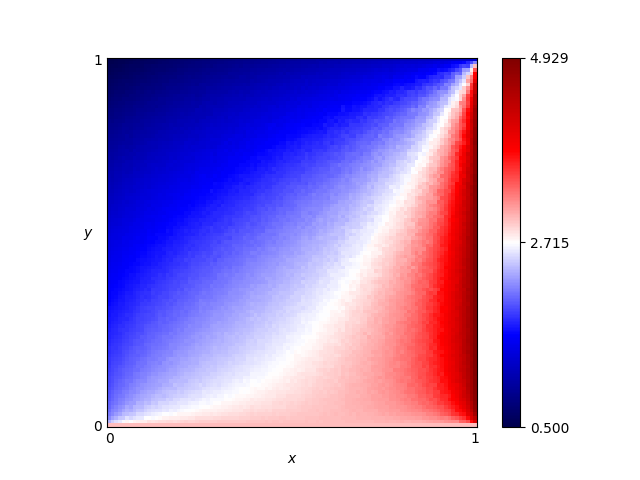
\includegraphics[height=.3\textheight]{./assets/images/Win-Stay_Lose-Shift.png}
    \caption{Pavlov fingerprinting with Tit for Tat used as the probe strategy.
    Figure was generated using~\cite{axelrodproject}.}
    \label{fig:fingerprinting}
\end{figure}

This section covered structured strategies and training methods. In the following
section software that has been developed with main aim simulating the IPD
is presented.

\subsection{Software}\label{section:software}

The research of the IPD heavily relays on software.
This is to be expected as the pioneer computer tournaments have become the main
means of simulating the interactions in an IPD game.
Many academic fields suffer from the lack of source code availability and the PD
is not an exception. Several of the tournaments that have been discussed so far were generated
using computer code, though not all of the source code was made available by the authors.
The code for Axelrod's original tournament is known to be lost and
moreover for the second tournament the only source code available is the code
for the 62 strategies (found on Axelrod's personal website~\cite{fortan_code}).

Several projects, however, are open, available and have been used as research
tools or educational platforms over the years. Two research tools are briefly
mentioned here~\cite{prison, axelrodproject} and two educational
tools~\cite{pd_trust, pd_game}. Both~\cite{prison, axelrodproject} are open
source projects used as research tools. PRISON is written in the programming
language Java and preliminary version was launched on 1998. It was used by it's
authors in several publications, such as~\cite{Beaufils1997}, which introduced
Gradual, and~\cite{Beaufils1988}. The project includes a good number of
strategies from the literature but unfortunately the last update of the project
dates back in 2004. Axelrod-Python is a software used
by~\cite{Knight2017,KnightHGC17, Goodman2018, Wang2017}. It is written in the
programming language Python following best practice approaches and contains the
largest collection of strategies, known to the author. The strategy list of
the project has been cited by publications~\cite{Anastassacos2018, Hayes2017,
Neumann2018}.

The ``Game of Trust"~\cite{pd_trust} is an on-line, graphical user interface
educational platform for learning the basics of game theory, the IPD
and the notion of strategies. It attracted a lot of attention
due to being ``well-presented with scribble-y hand drawn
characters''~\cite{trust_blogb} and ``a whole heap of fun''~\cite{trust_bloga}.
Finally~\cite{pd_game} is a personal project written in PHP. It's graphical user
interface that offers a big collection of strategies and allows the user to try
several matches and tournament configurations.

\subsection{Conclusion and Contemporary research}\label{section:contemporary_period}

This section of the paper served as a review of publications on the PD.
This review has partitioned the literature into five different sections,
focusing on different aspects of the research. Section~\ref{section:origin}
covered the early years of research. This was when simulating turns of the game
was only possible with human subject research.
Following the early years, the pioneer tournaments of Axelord were introduced in
Section~\ref{subsection:intelligent_design}. Axelrod's work offered the field an
agent based game theoretic framework to study the IPD.
In his original papers he asked researchers to design strategies to test their
performance with the new framework. The winning strategy of both his tournaments
was Tit for Tat. The strategy however came with limitations which were explored
by other researchers, and new strategies of intelligent design were introduced in
order to surpass Tit for Tat with some contributions such as Pavlov and Gradual.

Soon researchers came to realise that strategies should not just do well in a tournament setting
but should also be evolutionary robust. Evolutionary dynamics methods were
applied to many works in the field, and factors under which cooperation
emerges were explored, as described in Section~\ref{subsection:evolutionary_dynamics}.
This was not done only for unstructured populations, where all strategies
in the population can interact with each other, but also in population where
interactions were limited to only strategies that were close to each other.
In such topologies it was proven that even in the one shot game cooperation can
indeed emerge.

Evolutionary approaches can offer many insights in the study of the PD. In
evolutionary settings strategies can learn to adapt and take over population by
adjusting their actions; such algorithms can be applied so that evolutionarily
robust strategies can emerge. Algorithms and structures used to train strategies
in the literature were covered in Section~\ref{section:structured_strategies}.
From these training methods several strategies can emerge,
and to be able to differentiate between strategies the method fingerprinting was
introduced. The research of best play and cooperation has been going on since
the 1950s, and for simulating the game software has been developed along the
way. Few research and educational software have been briefly discussed
in Section~\ref{section:software}.

The study of the PD is still an ongoing field of pioneer and
innovating research where new variants and new structures of strategies are
continuously being explored~\cite{Ohtsuki2018}. The game now serves as a model
in a wide range of applications, for example in medicine and the study of cancer
cells~\cite{archetti2018, Kaznatchee2017}, as well as in social situations and
how they can be driven by rewards~\cite{Dridi2018}. New research is still ongoing
on the topics/trend covered in each section of this literature review,
for example on evolutionarily dynamics on graphs~\cite{Allen2017, hathcock2018,
Liu2017}.

A large scale of articles has been covered in each of the corresponding sections
of this review. This literature doe not pretend to have covered all the publications
in the field. It will soon in the following section that the field has had many
publications, exceeding 3000 articles. However, several important milestones
of the field have been presented here.

\section{Analysing a large corpus of articles}\label{section:analysis}

The focus of Section~\ref{section:timeline} has been to review academic
publications on the topic of the IPD. Whilst in
Section~\ref{section:timeline} several publications of specific interest were
covered and the literature was manually partitioned in different sections, in
the second part of this paper the publications are analysed using a large
dataset of articles.

In Section~\ref{section:background} some background research on bibliometrics is
discussed. The data collection process is covered in Section
\ref{section:data_collection} and a preliminary analysis of the data is
conducted in Section~\ref{section:preliminary_analysis}. In
Section~\ref{section:methodology}, the methodology which will be used to analyse
the author relationships is presented, that is graph theoretical methods used to
ascertain the level of collaborative nature of the field and identify influence.
This type of analysis has been carried out in~\cite{Liu2015}. The novelty here
is to consider approaches not considered in~\cite{Liu2015} such as the
centrality measures of the network, and apply them to a new dataset. A further
comparison of the results are made, relative to two other sub fields of game
theory: auction games~\cite{menezes2005} and the price of
anarchy~\cite{roughgarden2005} and a temporal analysis. Finally in
Section~\ref{section:results}, the results of the analysis are presented.

\subsection{Background}\label{section:background}

As discussed in~\cite{youngblood2018}, bibliometrics (the statistical analysis
of published works originally described by~\cite{pritchard1969}) has been used
to support historical assumptions about the development of fields
\cite{raina1998}, identify connections between scientific growth and policy
changes \cite{das2016}, develop a quantitative understanding of author
order~\cite{sekara2018}, and investigate the collaborative structure of an
interdisciplinary field~\cite{Liu2015}. Most academic research is undertaken in
the form of collaborative effort and as~\cite{Kyvik2017} points out, it is
rational that two or more people have the potential to do better as a group
than individually. Collaboration in groups has a long tradition in experimental
sciences and it has be proven to be productive according
to~\cite{Etzkowitz1992}. The number of collaborations can be very different
between research fields and understanding how collaborative a field is not
always an easy task. Several studies tend to consider academic citations as a
measure for these things. A blog post published by Nature~\cite{nature_blog}
argues that depending on citations can often be misleading because the true
number of citations can not be known. Citations can be missed due to data entry
errors, academics are influenced by many more papers than they actually cite and
several of the citations are superficial.

A more recent approach to measure collaborative behaviour is to use the co
authorship network, as described in~\cite{Liu2015}. Using this approach has many
advantages as several graph theoretic measures can be used as proxies to explain
authors relationship. In~\cite{Liu2015}, they analyse the development of the
field ``evolution of cooperation'' using this approach. The topic ``evolution of
cooperation'' is a multidisciplinary field which also includes a large number of
publications on the PD. This paper builds upon the work done
by~\cite{Liu2015} and extends their methodology. Though in \cite{Liu2015}, they
considered a data set from a single source, Web of Science, the data set
described here has been collected from five different sources. Moreover, the
collaborative results of the analysis are compared to those of two different sub
fields.

Co authorship networks have also been used in~\cite{youngblood2018} for
classifying topics of an interdisciplinary field. This was done using centrality
measures, which will be covered in Section~\ref{section:data_collection}, here
centrality measures are used in order to understand the influence an author can
have and can receive by being part of an academic group. Furthermore,
in~\cite{alshebli2018} they look at the relationship between research impact and
five classes of diversity: ethnicity, discipline, gender, affiliation, and
academic age. These characteristics of the authors are not being captured here.
In future work these characteristics would be included in the analysis.

\subsection{Data Collection}\label{section:data_collection}

Academic articles are accessible through scholarly databases. Several databases
and collections today offer access through an open application protocol
interface (API). An API allows users to query directly a journal's database and
bypass the graphical user interface. Interacting with an API has two phases:
requesting and receiving. The request phase includes composing a url with the
details of the request. For example,
\url{http://export.arxiv.org/api/query?search_query=abs:prisoner's
dilemma&max_results=1} represents a request message. The first part of the
request is the address of the API. In this example the address corresponds to
the API of arXiv. The second part of the request contains the search arguments.
In this example it is requested that the word `prisoners dilemma' exists within
the article's title. The format of the request message is different from API to
API. The receive phase includes receiving a number of raw metadata of articles
that satisfies the request message. The raw metadata are commonly received in
extensive markup language (xml) or Javascript object notation (json)
formats~\cite{nurseitov2009}. Similarly to the request message, the structure of
the received data differs from journal
to journal.

The data collection is crucial to this study. To ensure that this study can be
reproduced all code used to query the different APIs has been packaged as a
Python library and is available online~\cite{nikoleta_2017}. The software could
be used for any type of projects similar to the one described here,
documentation for it is available at:
\url{http://arcas.readthedocs.io/en/latest/}. Project~\cite{nikoleta_2017} allow
users to collect articles from a list of APIs by specifying just a single
keyword. Four prominent journals in the field and a pre print server were used
as sources to collect data for this analysis: PLOS, Nature, IEEE, Springer and
arXiv.

The following series of search terms were used to identify relevant articles:

\begin{itemize}
    \item ``prisoner's dilemma'',
    \item ``prisoners dilemma'',
    \item ``prisoner dilemma'',
    \item ``prisoners evolution'',
    \item ``prisoner game theory''
\end{itemize}

and articles for which any of these terms existed within the title, the abstract
or the text are included in the analysis. More specifically, 23\% of article
considered here were included because any of the above terms existed within the
abstract, 50\% within the main text and 27\% within the title. As will be
described in Section~\ref{section:preliminary_analysis}, two other game
theoretic sub fields auction games and the price of anarchy were also considered
in this work. For collecting data on these sub fields the search terms used were
``auction game theory'' and ``price of anarchy''. The three data sets are
archived and available at~\cite{auction_data_2018, anarchy_data_2018,
pd_data_2018}. Note that the latest data collection was performed on \(30^{\text{th}}\)November 2018.
% TODO Ensure this stay accurate

\subsection{Preliminary Analysis}\label{section:preliminary_analysis}

A summary of each of the three data sets used is presented in this section.
The three data sets are:

\begin{itemize}
    \item The main data set which contains articles on the prisoner's dilemma~\cite{pd_data_2018}.
    \item A data set which contains article on auction games~\cite{auction_data_2018}.
    \item A data set which contains articles on the price of anarchy~\cite{anarchy_data_2018}.
\end{itemize}

The main data set is archived at~\cite{pd_data_2018}. It
consists of \totalarticles articles with unique titles. In case of duplicates
the preprint version of an article (collected from arXiv) was dropped.
Of these \totalarticles article, \manual have not been collected from the
aforementioned APIs. These articles were of specific interest and manually added
to the dataset throughout the writing of Section~\ref{section:timeline}. A
similar approach was used in~\cite{Liu2015} where a number of articles of interest
where manually added to the data set. A more
detailed summary of the articles' provenance is given by Table~\ref{table:provenance}.
Only 3\% of the data set consists of articles that were manually added and 34\% of the
articles were collected from arXiv.

\begin{table}[!hbtp]
    \begin{center}
    \begin{tabular}{lrr}
\toprule
{} &  \# of Articles &  Percentage \\
provenance &                &             \\
\midrule
Manual     &             89 &        2.92 \\
IEEE       &            295 &        9.67 \\
Springer   &            458 &       15.01 \\
PLOS       &            482 &       15.79 \\
Nature     &            673 &       22.05 \\
arXiv      &           1055 &       34.57 \\
\bottomrule
\end{tabular}

    \end{center}
    \caption{Articles' provenance for the main data set~\cite{pd_data_2018}.}
    \label{table:provenance}
\end{table}

The average number of publications was calculated for the entire dataset and for
each provenance. The average number of publications is denoted as, \(\mu_P =
\frac{N_A}{N_Y},\) where \(N_A\) is the total number of articles and \(N_Y\) is
the years of publication. The years of publication is calculated as the range
between the collection date and the first published article, for each
provenance, within the data. These averages are summarised in
Table~\ref{table:publication_rates}. Overall an average of 49 articles are
published per year on the topic. The most significant contribution to this
appears to be from arXiv with 16 articles per year, followed by Nature with 10
and Springer with 9.

\begin{table}[!hbtp]
    \begin{center}
    \begin{tabular}{lr}
\toprule
{} &  Av. Yearly publication \\
\midrule
IEEE     &                     5.0 \\
PLOS     &                     8.0 \\
Springer &                     9.0 \\
Nature   &                    11.0 \\
arXiv    &                    16.0 \\
Overall  &                    49.0 \\
\bottomrule
\end{tabular}

    \end{center}
    \caption{Average yearly publication $(\mu_P)$ for main data set~\cite{pd_data_2018}.}
    \label{table:publication_rates}
\end{table}

Though the average publication offers insights about the publications of the
fields, it remains a constant number. The data handled here is a time
series from 1950, when the game was introduced, until 2018 (Figure~\ref{fig:timeseries}). 
Two observations can be made from Figure~\ref{fig:timeseries}.

\begin{enumerate}
    \item There is a steady increase to the number of publications since the
    1980s and the introduction of computer tournaments.
    \item There is a decrease in 2017-2018. This is due to our data set being
    incomplete. Articles that have been written in 2017-2018 have either not
    being published or were not retrievable by the APIs by the time of writing
    this manuscript.
\end{enumerate}

These observations can be confirmed by studying the time series.
Using~\cite{scipy}, an exponential distribution is fitted to the data from
1980-2016. The exponential fit demonstrates that since 1980 there has been an
increase in the number of publications until 2016 (Figure~\ref{fig:fitting}).
The fitted model can also be used to forecast the behaviour of the field for the
next 5 years. The forecasted periods are plotted in
Figure~\ref{fig:forecasting}. The time series has indicated a slight decrease
however the model forecasts that the number of publications will keep
increasing, thus indicating that the field of the iterated prisoner's dilemma
still attracts academic attention.

\begin{figure}[!hbtp]
\begin{minipage}{.45\textwidth}
    \centering
    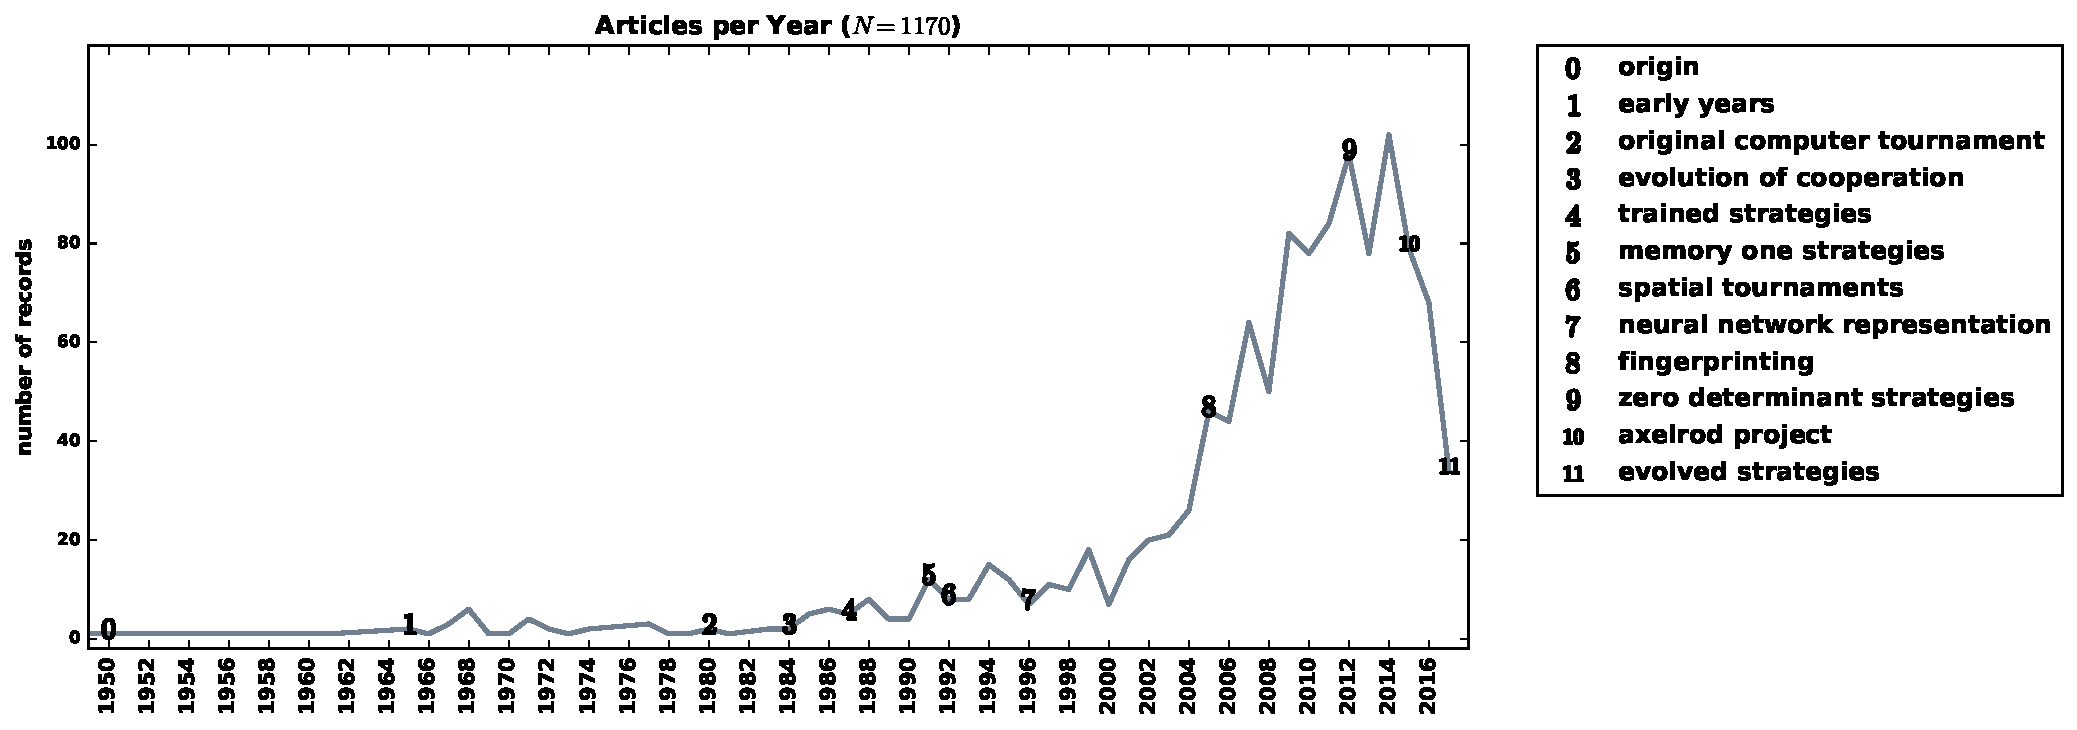
\includegraphics[width=.9\textwidth]{./assets/images/timeline.pdf}
    \caption{Line plot; \# of articles published on the PD 1950-2019.}\label{fig:timeseries}
\end{minipage}
\begin{minipage}{.45\textwidth}
    \centering
    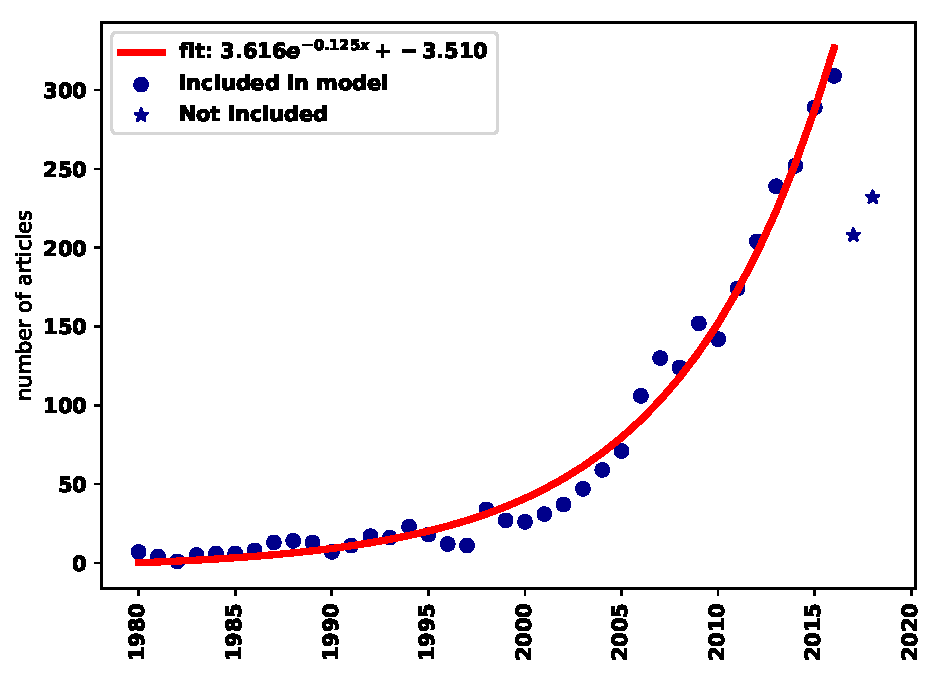
\includegraphics[width=.9\textwidth]{./assets/images/fitting.pdf}
    \caption{Scatter plot; \# of articles published on the PD 1980-2019.}\label{fig:fitting}
\end{minipage}
\end{figure}

\begin{figure}[!hbtp]
    \centering
    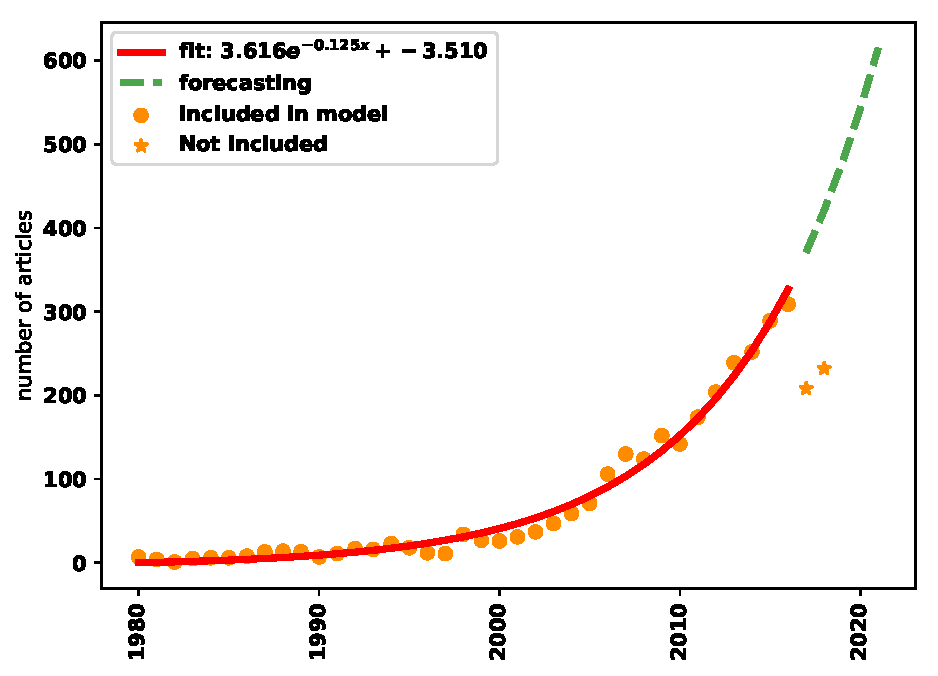
\includegraphics[width=.5\textwidth]{./assets/images/forecasting.pdf}
    \caption{Forecast for 2017-2022.}\label{fig:forecasting}
\end{figure}

To allow for a comparative analysis two sub fields of game theory have been chosen
for this work; auction games and the price of anarchy.

\begin{itemize}
    \item Auction theory is a branch of game theory which researches the
    properties of auction markets. Game theory has been used for years to study
    auctions and the behaviour of bidders~\cite{Shubik1971}. The earliest entry
    in our data set~\cite{auction_data_2018} goes back to 1974
    (Figure~\ref{fig:timeseries_ag}). Note that no articles have been added
    manually for auction games.
    \item Price of Anarchy is a concept in game theory which measures how the
    efficiency of a system degrades due to selfish behaviour of it's agents.
    There is a variety of such measures however the price of anarchy has
    attracted a lot of attention since it's informal introduction in 1999
    by~\cite{Koutsoupias1999}. Note that~\cite{Koutsoupias1999} has been
    manually added to the date set~\cite{anarchy_data_2018} and it's the first entry
    (Figure~\ref{fig:timeseries_pa}).
\end{itemize}

A summary of both data sets, in comparison to that of~\cite{pd_data_2018}, is
given by Table~\ref{table:summary_other_topics}.

\begin{table}[!hbtp]
    \centering
    \resizebox{\textwidth}{!}{
    \begin{tabular}{lrrllrrrrr}
\toprule
{} &  Num. Articles &  Num. Authors & Manual (\%) & PLOS (\%) &  Nature (\%) &  Springer (\%) &  IEEE (\%) &  arXiv (\%) &  Av. Yearly Publication \\
\midrule
Prisoner's Dilemma &           3089 &          5811 &       2.88 &     15.6 &       21.79 &         18.52 &      9.55 &      34.19 &                     NaN \\
Auction Games      &           3444 &          5362 &          - &        - &        5.89 &         37.63 &      7.46 &      51.36 &                     NaN \\
Price of Anarchy   &            746 &          1314 &          - &     1.74 &       24.66 &         38.07 &     30.70 &       8.85 &                     NaN \\
\bottomrule
\end{tabular}
}
    \caption{Measures of all three data sets.}\label{table:summary_other_topics}
\end{table}

The IPD and auction theory are popular topics and have
been studied for decades. A large number of articles have
been collected for both topics, \totalarticles and 3444 respectively. Though, auction
games have a larger number of articles, the IPD
has almost 300 more authors.

Auction games have an overall average yearly publication
of 93 articles per year compared to the PD with 49 per year. The 50\% of articles
for auction games have been collected from the pre print server arXiv and no articles have
been published in PLOS.

Compared to these two topics the price of anarchy is a fairly recent one. Only a
total of 747 articles have been collected, however it has a large number
of 1229 authors. On average each paper has two authors. It has an overall average
yearly publication rate of 39 articles and the biggest contribution has been made
to Springer (37\%).

\begin{figure}[!hbtp]
    \begin{minipage}{.45\textwidth}
        \centering
        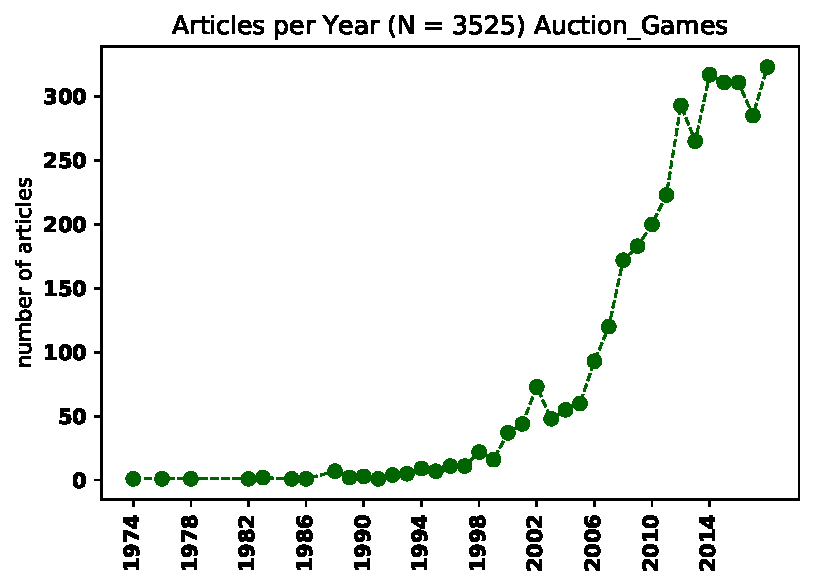
\includegraphics[width=\textwidth]{./assets/images/Auction_Games.pdf}
        \caption{Line plot; \# articles published on auction games 1974-2018.}\label{fig:timeseries_ag}
    \end{minipage}%
    \begin{minipage}{.45\textwidth}
        \centering
        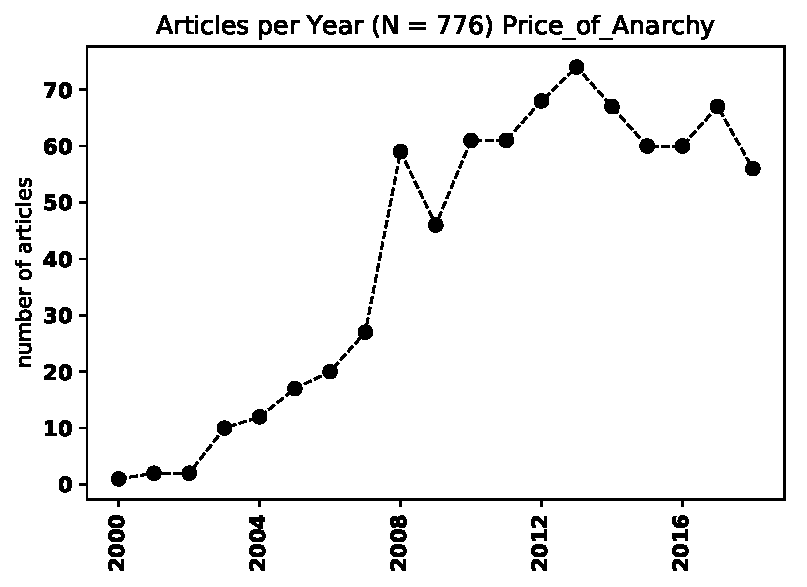
\includegraphics[width=\textwidth]{./assets/images/Price_of_Anarchy.pdf}
        \caption{Line plot; \# articles published on the price of anarchy.}\label{fig:timeseries_pa}
    \end{minipage}
    \end{figure}

\subsection{Methodology}\label{section:methodology}

The relationship between the authors within a field will be modelled as a graph
\(G = (V_G, E_G)\) where \(V_G\) is the set of nodes and \(E_G\)  is the set of
edges. The set \(V_G\) represents the authors and an edge connects two authors
if and only if those authors have written together. The co authorship network is
constructed using the main data set described in
Section~\ref{section:preliminary_analysis} and the open source package
\cite{networkx}. The PD network is denoted as \(G_1\) where the
number of unique authors \(|V(G_1)|\) is \authors and \(|E(G_1)|\) is 10397.
All authors' names were formatted as their last name and first initial (i.e.
Martin A. Nowak to Martin Nowak). This was done to avoid errors such as Martin
A. Nowak and Martin Nowak, being treated as a different person.

Collaborativeness, will be analysed using measures such as, isolated nodes,
connected components, clustering coefficient, communities, modularity and average degree.
These measures show the number of connections authors can have
and how strongly connected these people are. The number of isolated nodes is the
number of nodes that are not connected to another node, thus the
number of authors that have published alone. The average degree denotes the average
number of neighbours for each nodes, i.e. the average number of collaborations
between the authors.

A connected component is a maximal set of nodes such that each pair of nodes is
connected by a path. The number of connected components as well as the size of the
largest connected component in the network are reported.
The size of the largest connected component represents the scale of the central cluster
of the entire network, as it will discussed in the analysis section.
Clustering coefficient and modularity and are also calculated. The clustering
coefficient, defined as 3 times the number of triangle on the graph divided
by the number of connected triples of nodes, is a local measure of the degree to
which nodes in a graph tend to cluster together
in a clique. It is precisely the probability that the collaborators
of an author also write together.

In comparison, modularity is a global measure designed to measure the strength of
division of a network into communities. The number of communities will be reported
using the Clauset-Newman-Moore method~\cite{clauset2004}. Also the modularity index
is calculated using the Louvain method described in~\cite{Blondel2008}. The value
of the modularity index can vary between \([-1, 1]\), a high value of modularity
corresponds to a structure where there are dense connections between the nodes within
communities but sparse connections between nodes in different communities.
That means that authors in the network are mainly connected co-authors that they
all have written together, and not to several different collaborators.

Networks are commonly dominated by one person who controls information flow and
people that receive a great amount of information due to their position.
Two further points are aimed to be explored in this work, (1) which people control the flow;
as in which people influence the field the most and (2) which are the authors that
gain the most from the influence of the field. To measure these concepts graph
theoretic metrics, more specifically centrality measures are going to be used.
Centrality measures are often used to understand different
aspects fo social networks~\cite{Landherr2010}. Two centrality measures have been
chosen for this paper and these are closeness and betweenness centrality.

\begin{enumerate}
    \item In networks some nodes have a short distance to a lot of nodes and
    consequently are able to spread information on the network very effectively.
    A representative of this idea is \textbf{closeness centrality}, where a node
    is seen as centrally involved in the network if it requires only few
    intermediaries to contact others and thus is structurally relatively
    independent. Here, this is interpreted as influence. Authors with a high
    value of closeness centrality, are the authors that spread scientific
    knowledge easier on the network and they have high influence.
    \item Another centrality measure is the \textbf{betweenness centrality},
    where the determination of an author's centrality is based on the quotient
    of the number of all shortest paths between nodes in the network that
    include the node in question and the number of all shortest paths in the
    network. In betweenness centrality the position of the node matters. Nodes
    with a higher value of betweenness centrality are located in positions that
    a lot of information pass through them, this is interpreted as the gain from
    the influence, thus these authors gain the most from their networks.
\end{enumerate}

In the next section all the metrics discussed here are calculated for the data
sets in order to provide insights into the field.

\subsection{Analysis of co authorship network}\label{section:results}

As mentioned previously, \(G_1\) denotes the co authorship network of the
IPD. A graphical representation is given by
Figure~\ref{fig:g_one_network}. It is evident that the network is disjoint,
which is only natural as many authors write academic articles on their own. More
specifically, a total of \isolated authors, have had single author publications,
which corresponds to the \isolatedpercentage (\%) of authors in \(G_1\).

There are a total of \connectedcomponents connected components and the largest
one has a size of \largestcc nodes. The largest connected component is shown in
Figure~\ref{fig:g_one_cluster} and is going to be refereed to as the main
cluster of the network. There are total of \communities communities in \(G_1\).
The network has a clustering coefficient of 0.708, thus authors are 70\%
likely to write with a collaborator's co author and the degree distribution,
Figure~\ref{fig:degree_distrs}, shows that the average degree is approximately
\(4\). Thus authors are on average connected to 4 other authors, however there
are authors with far more connections, the largest one being 58.

In~\cite{Liu2015} the collaborative metrics for the ``evolution of cooperation''
co authorship network were reported. Though their network is of smaller size
(number of nodes 3670 \(<\) 5394), the collaborative metrics are fairly similar
between the two graphs (clustering coeff. \(0.632\) and modularity
0.950 close to 0.977), indicating that for the same multidisciplinary field the same
remarks can be made from a different co authors network. How do these compare to other fields
and more specifically to other fields of game theory?

The auction games network \(G_2\), and the price of anarchy network \(G_3\)
are given by Figures~\ref{fig:g_two} and~\ref{fig:g_three} and their respective
largest cluster in Figures~\ref{fig:g_two_cluster} and \ref{fig:g_three_cluster}.
As stated before \(G_3\) is the smallest network. \(G_2\) network appears to be
very similar to \(G_1\), however it's main cluster is larger in size.

\begin{figure}[!hbtp]
    \begin{subfigure}{.45\textwidth}\centering
        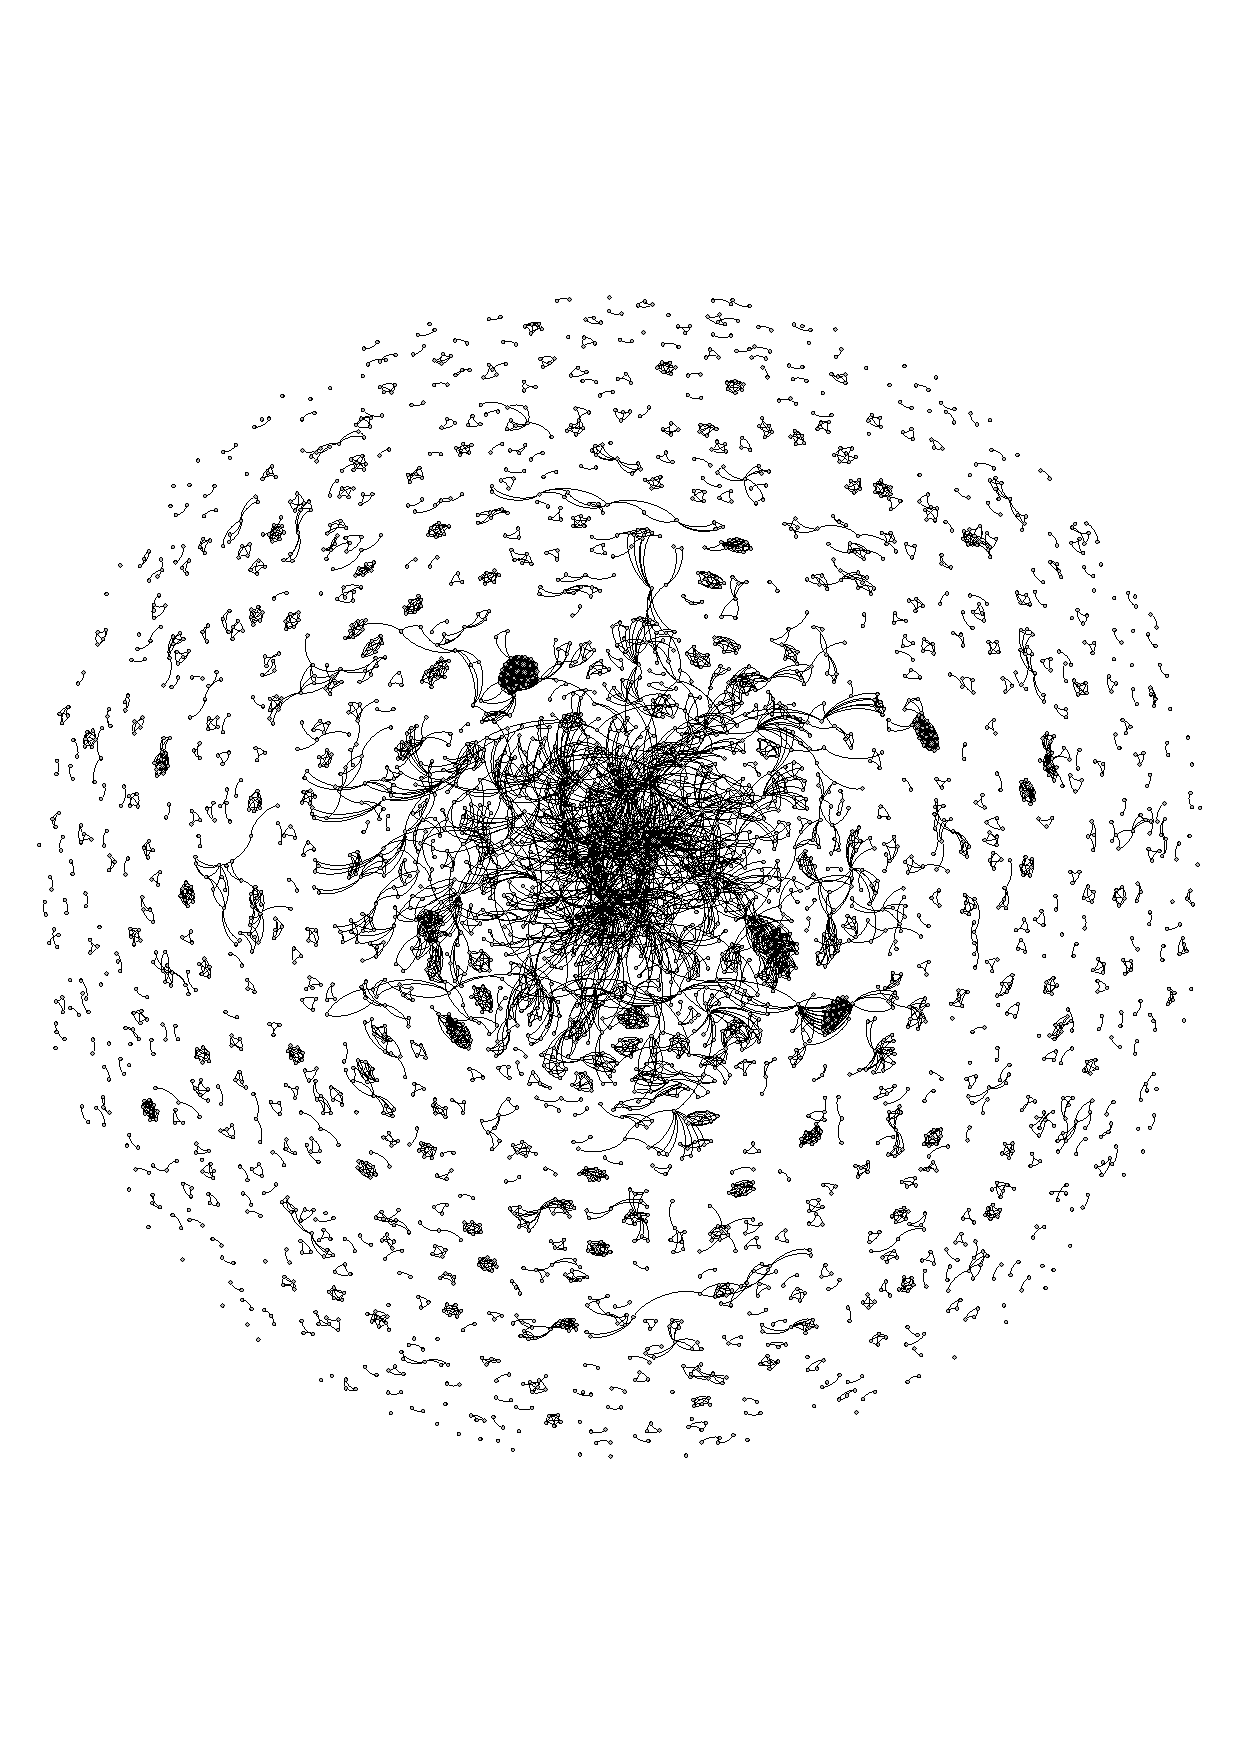
\includegraphics[width=.54\textwidth]{./assets/images/pd_network.pdf}
        \caption{\(G_1\) network.}\label{fig:g_one_network}
    \end{subfigure}
    \begin{subfigure}{.45\textwidth}\centering
        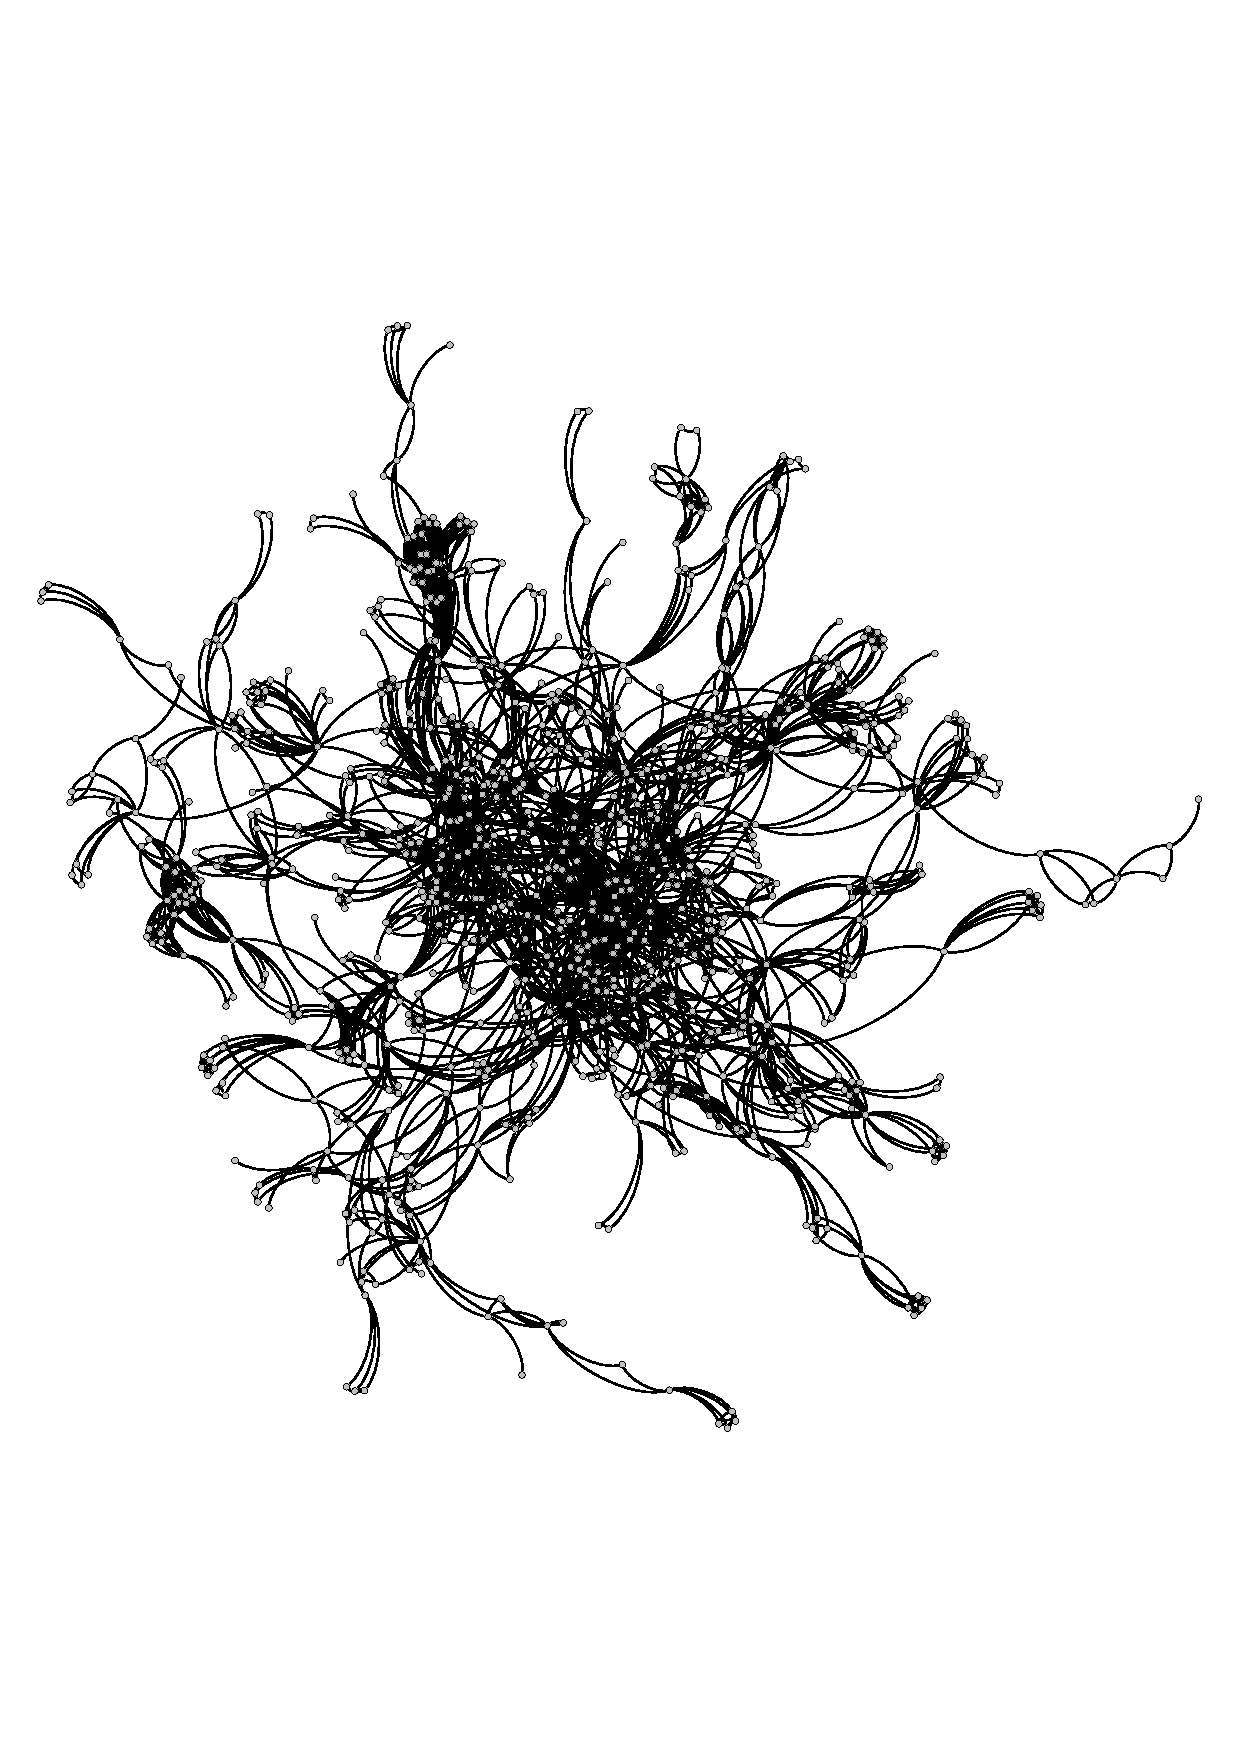
\includegraphics[width=.54\textwidth]{./assets/images/pd_network_cluster.pdf}
        \caption{\(G_1\) largest connected component, \(\bar{G}_{1}\).}\label{fig:g_one_cluster}
     \end{subfigure}
     
     \begin{subfigure}{.45\textwidth}\centering
        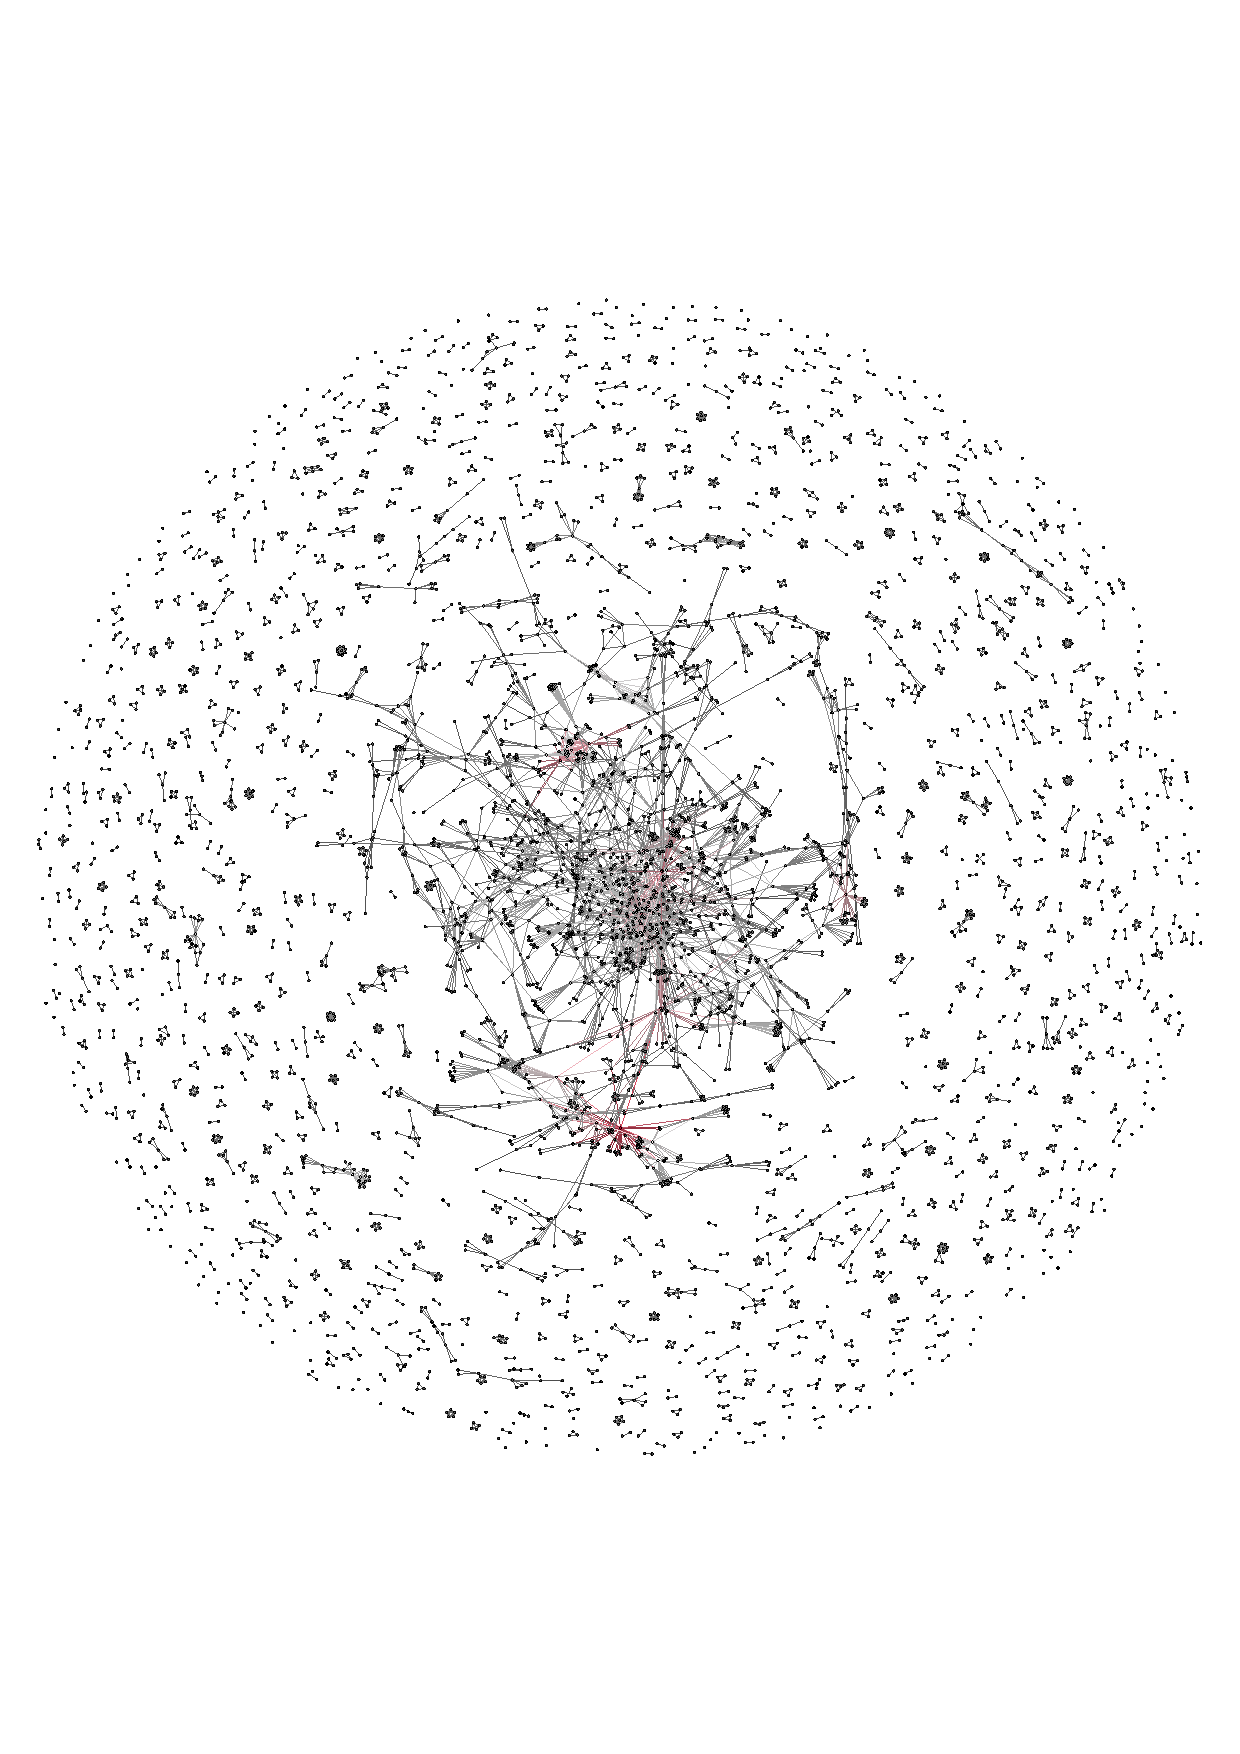
\includegraphics[width=.54\textwidth]{./assets/images/auction.pdf}
        \caption{\(G_2\) network.}\label{fig:g_two}
     \end{subfigure}
    \begin{subfigure}{.45\textwidth}\centering
        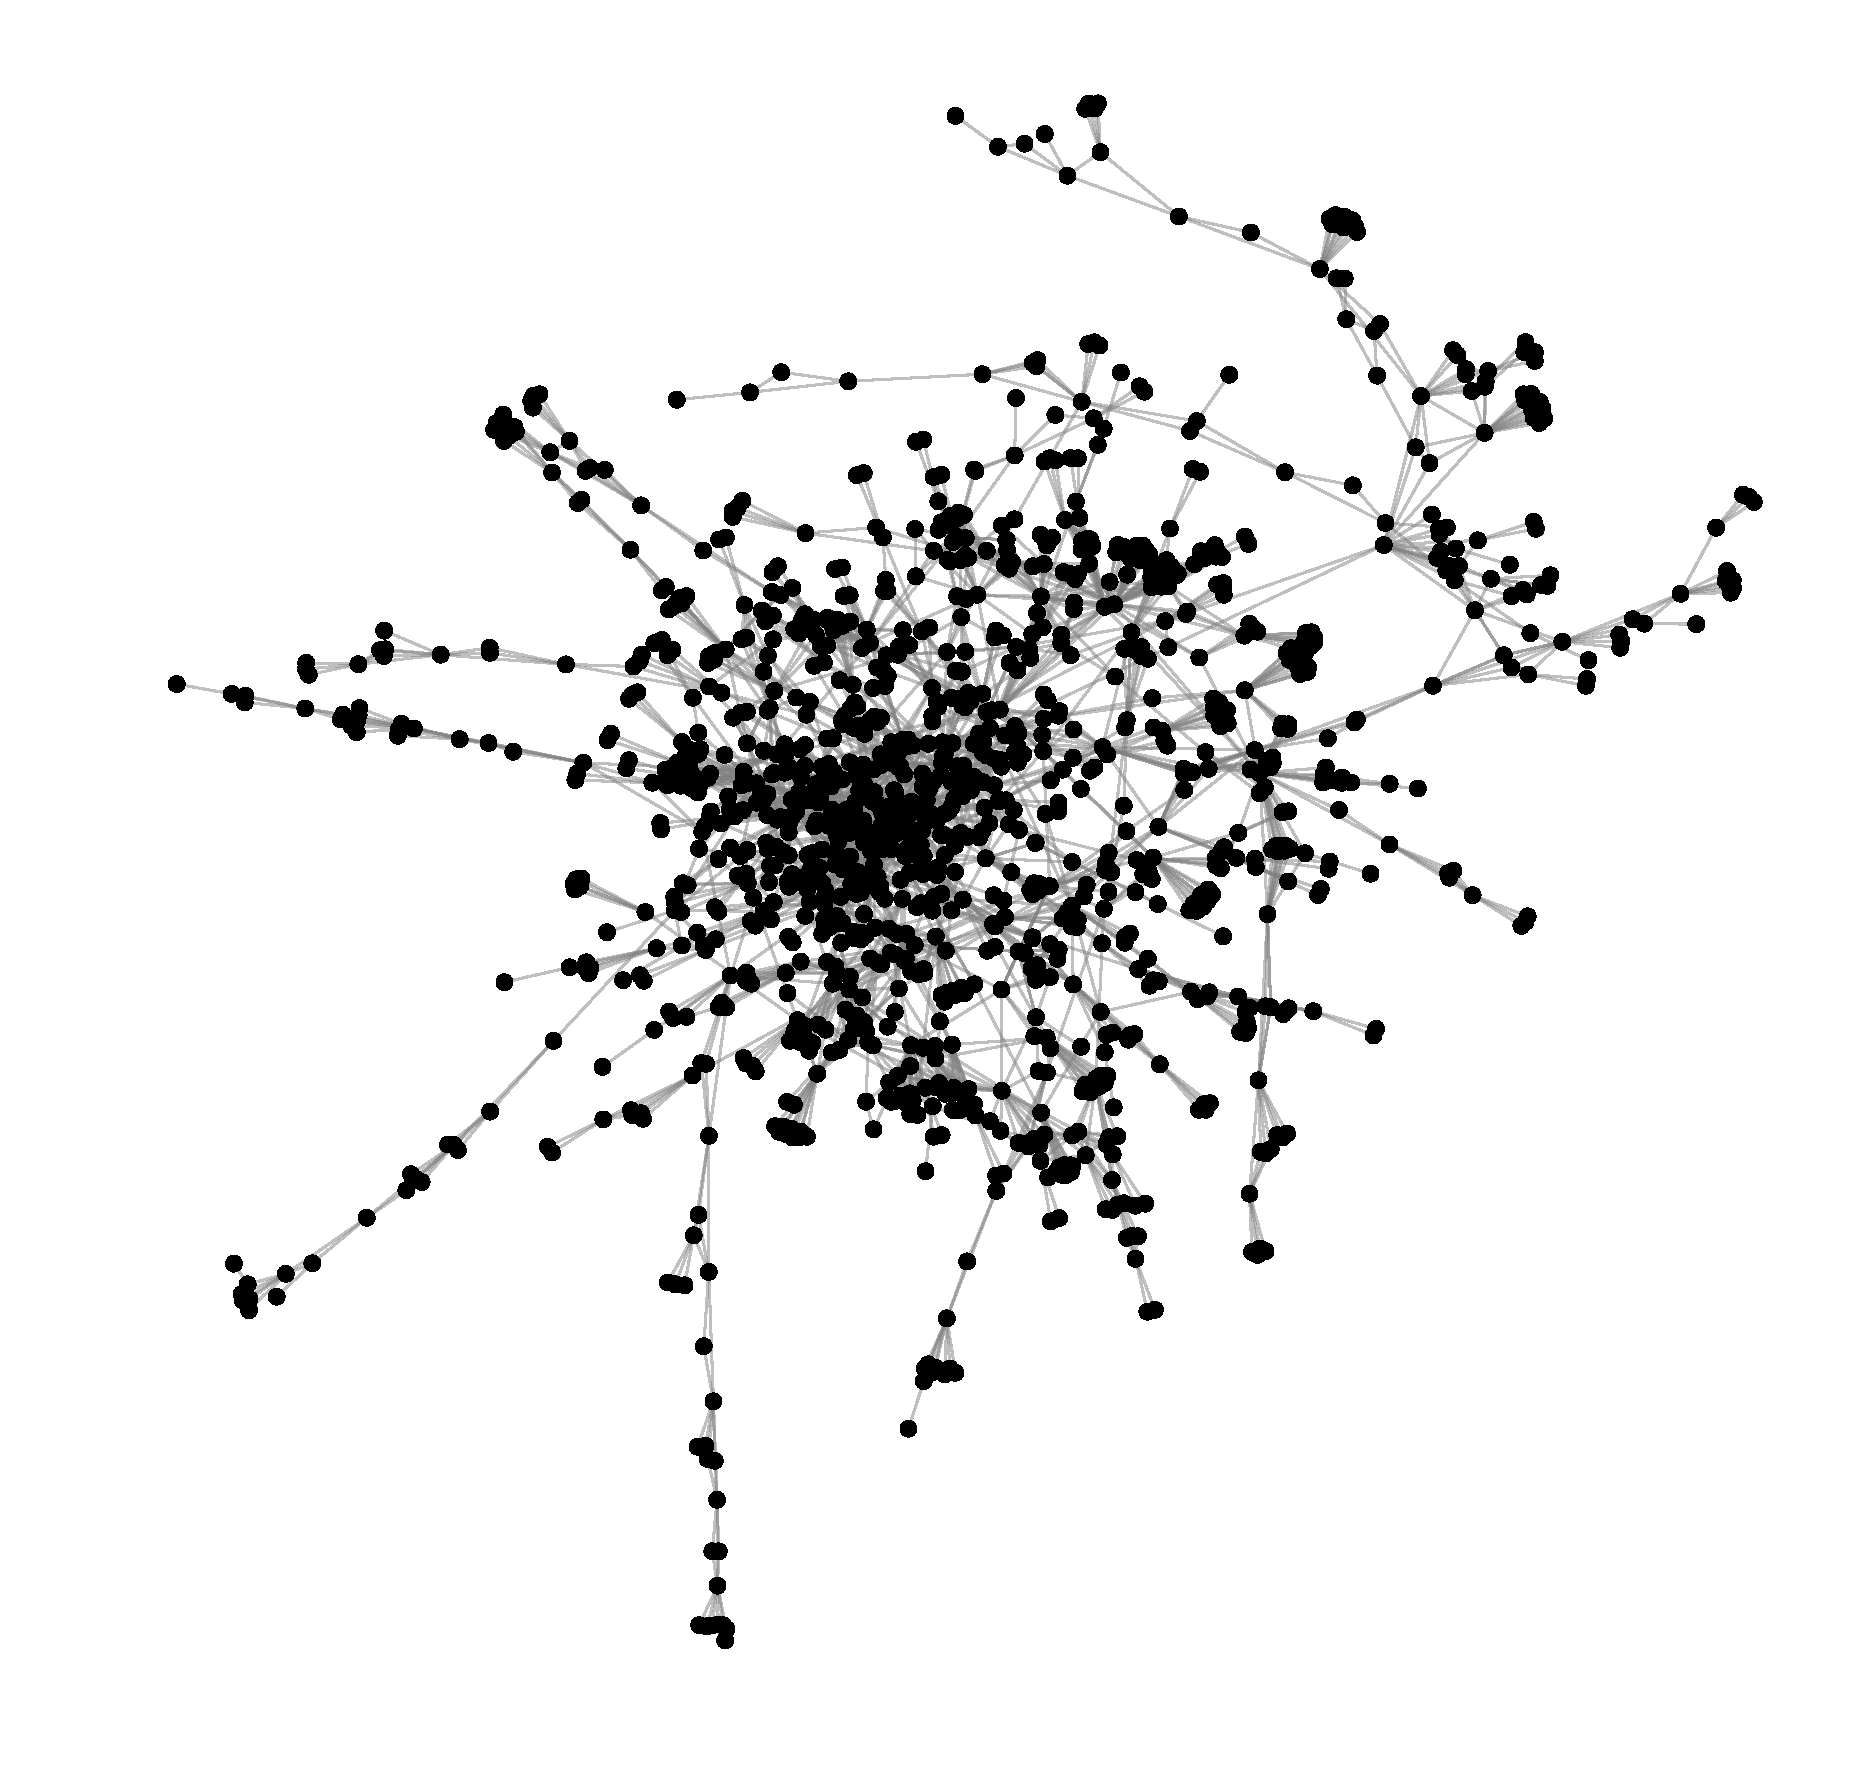
\includegraphics[width=.54\textwidth]{./assets/images/auction_network_cluster.pdf}
        \caption{\(G_2\) largest connected component,  \(\bar{G}_{2}\).}\label{fig:g_two_cluster}
    \end{subfigure}

    \begin{subfigure}{.45\textwidth}\centering
        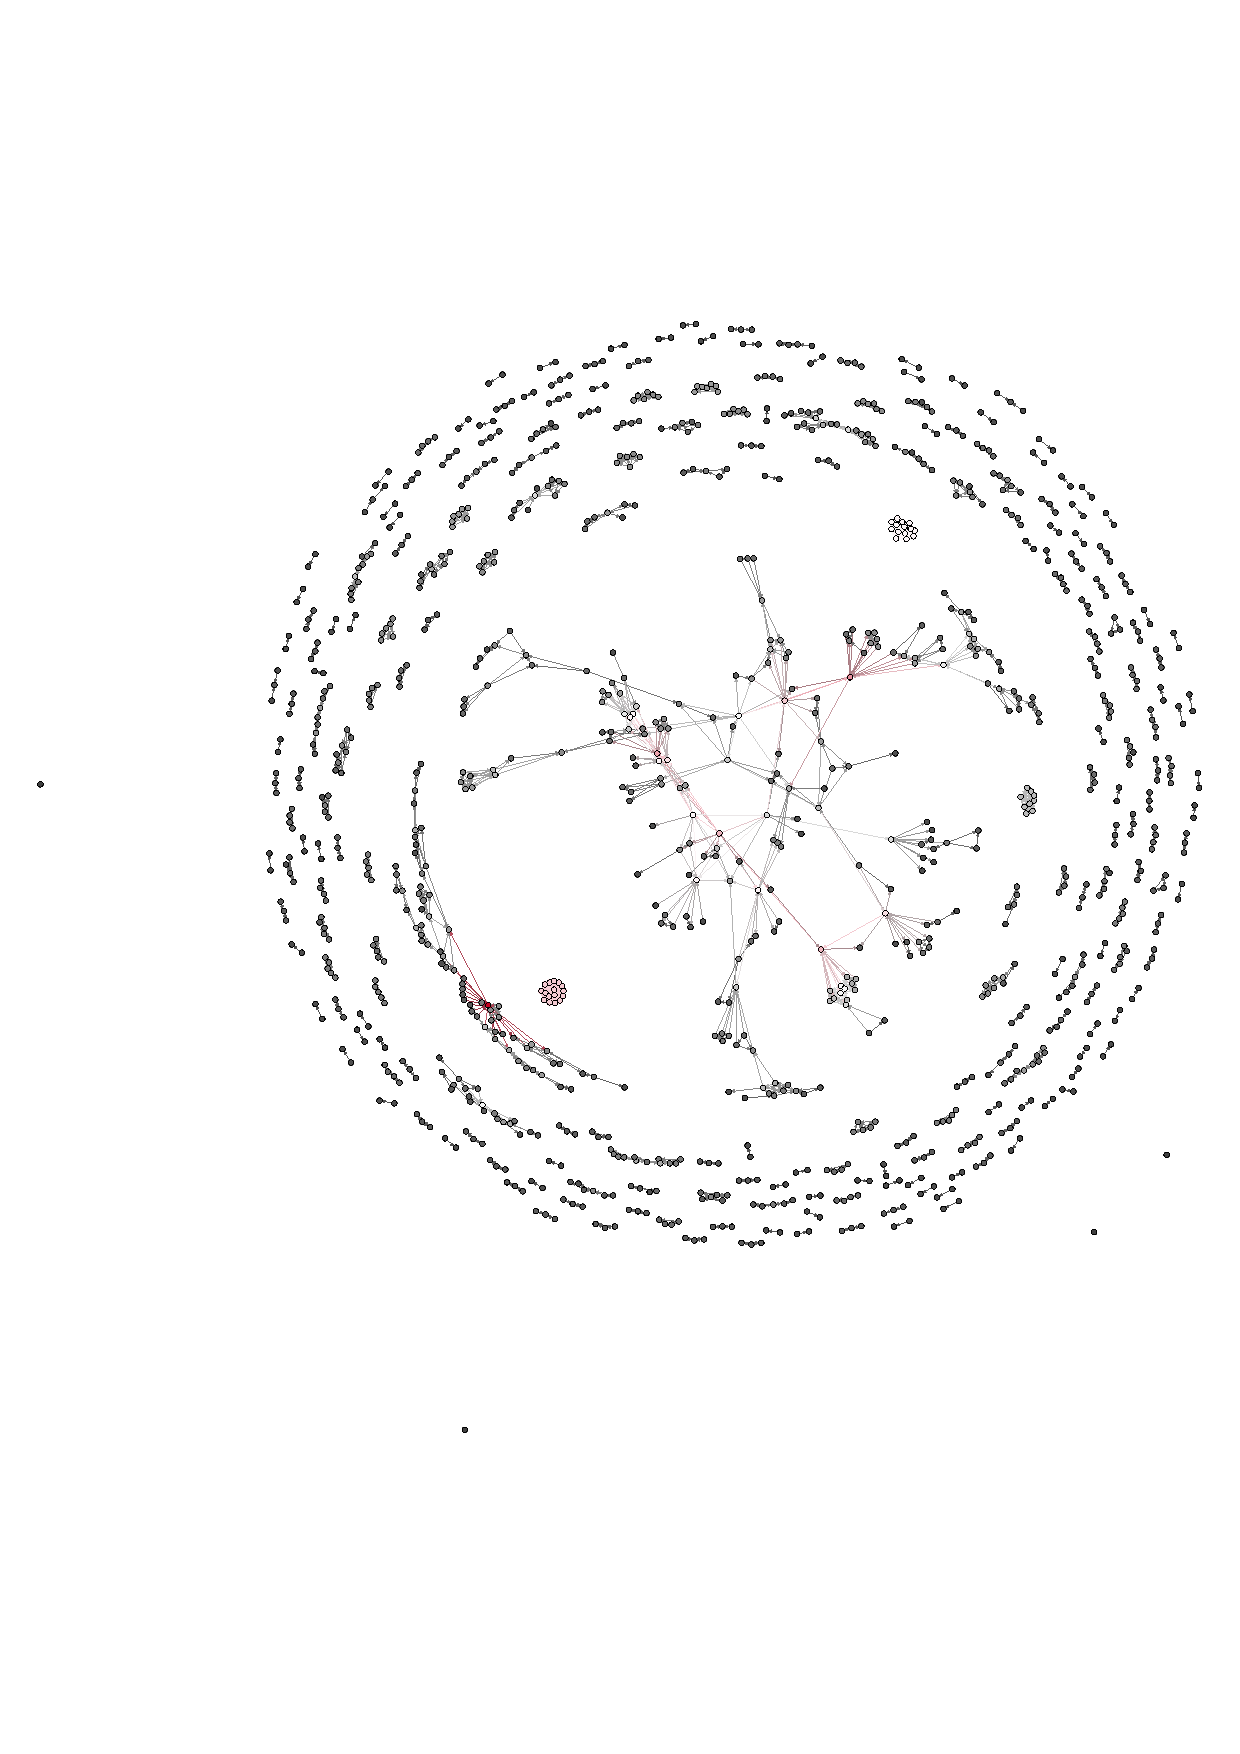
\includegraphics[width=.54\textwidth]{./assets/images/anarchy_network.pdf}
        \caption{\(G_3\) network.}\label{fig:g_three}
     \end{subfigure}
     \begin{subfigure}{.45\textwidth}\centering
        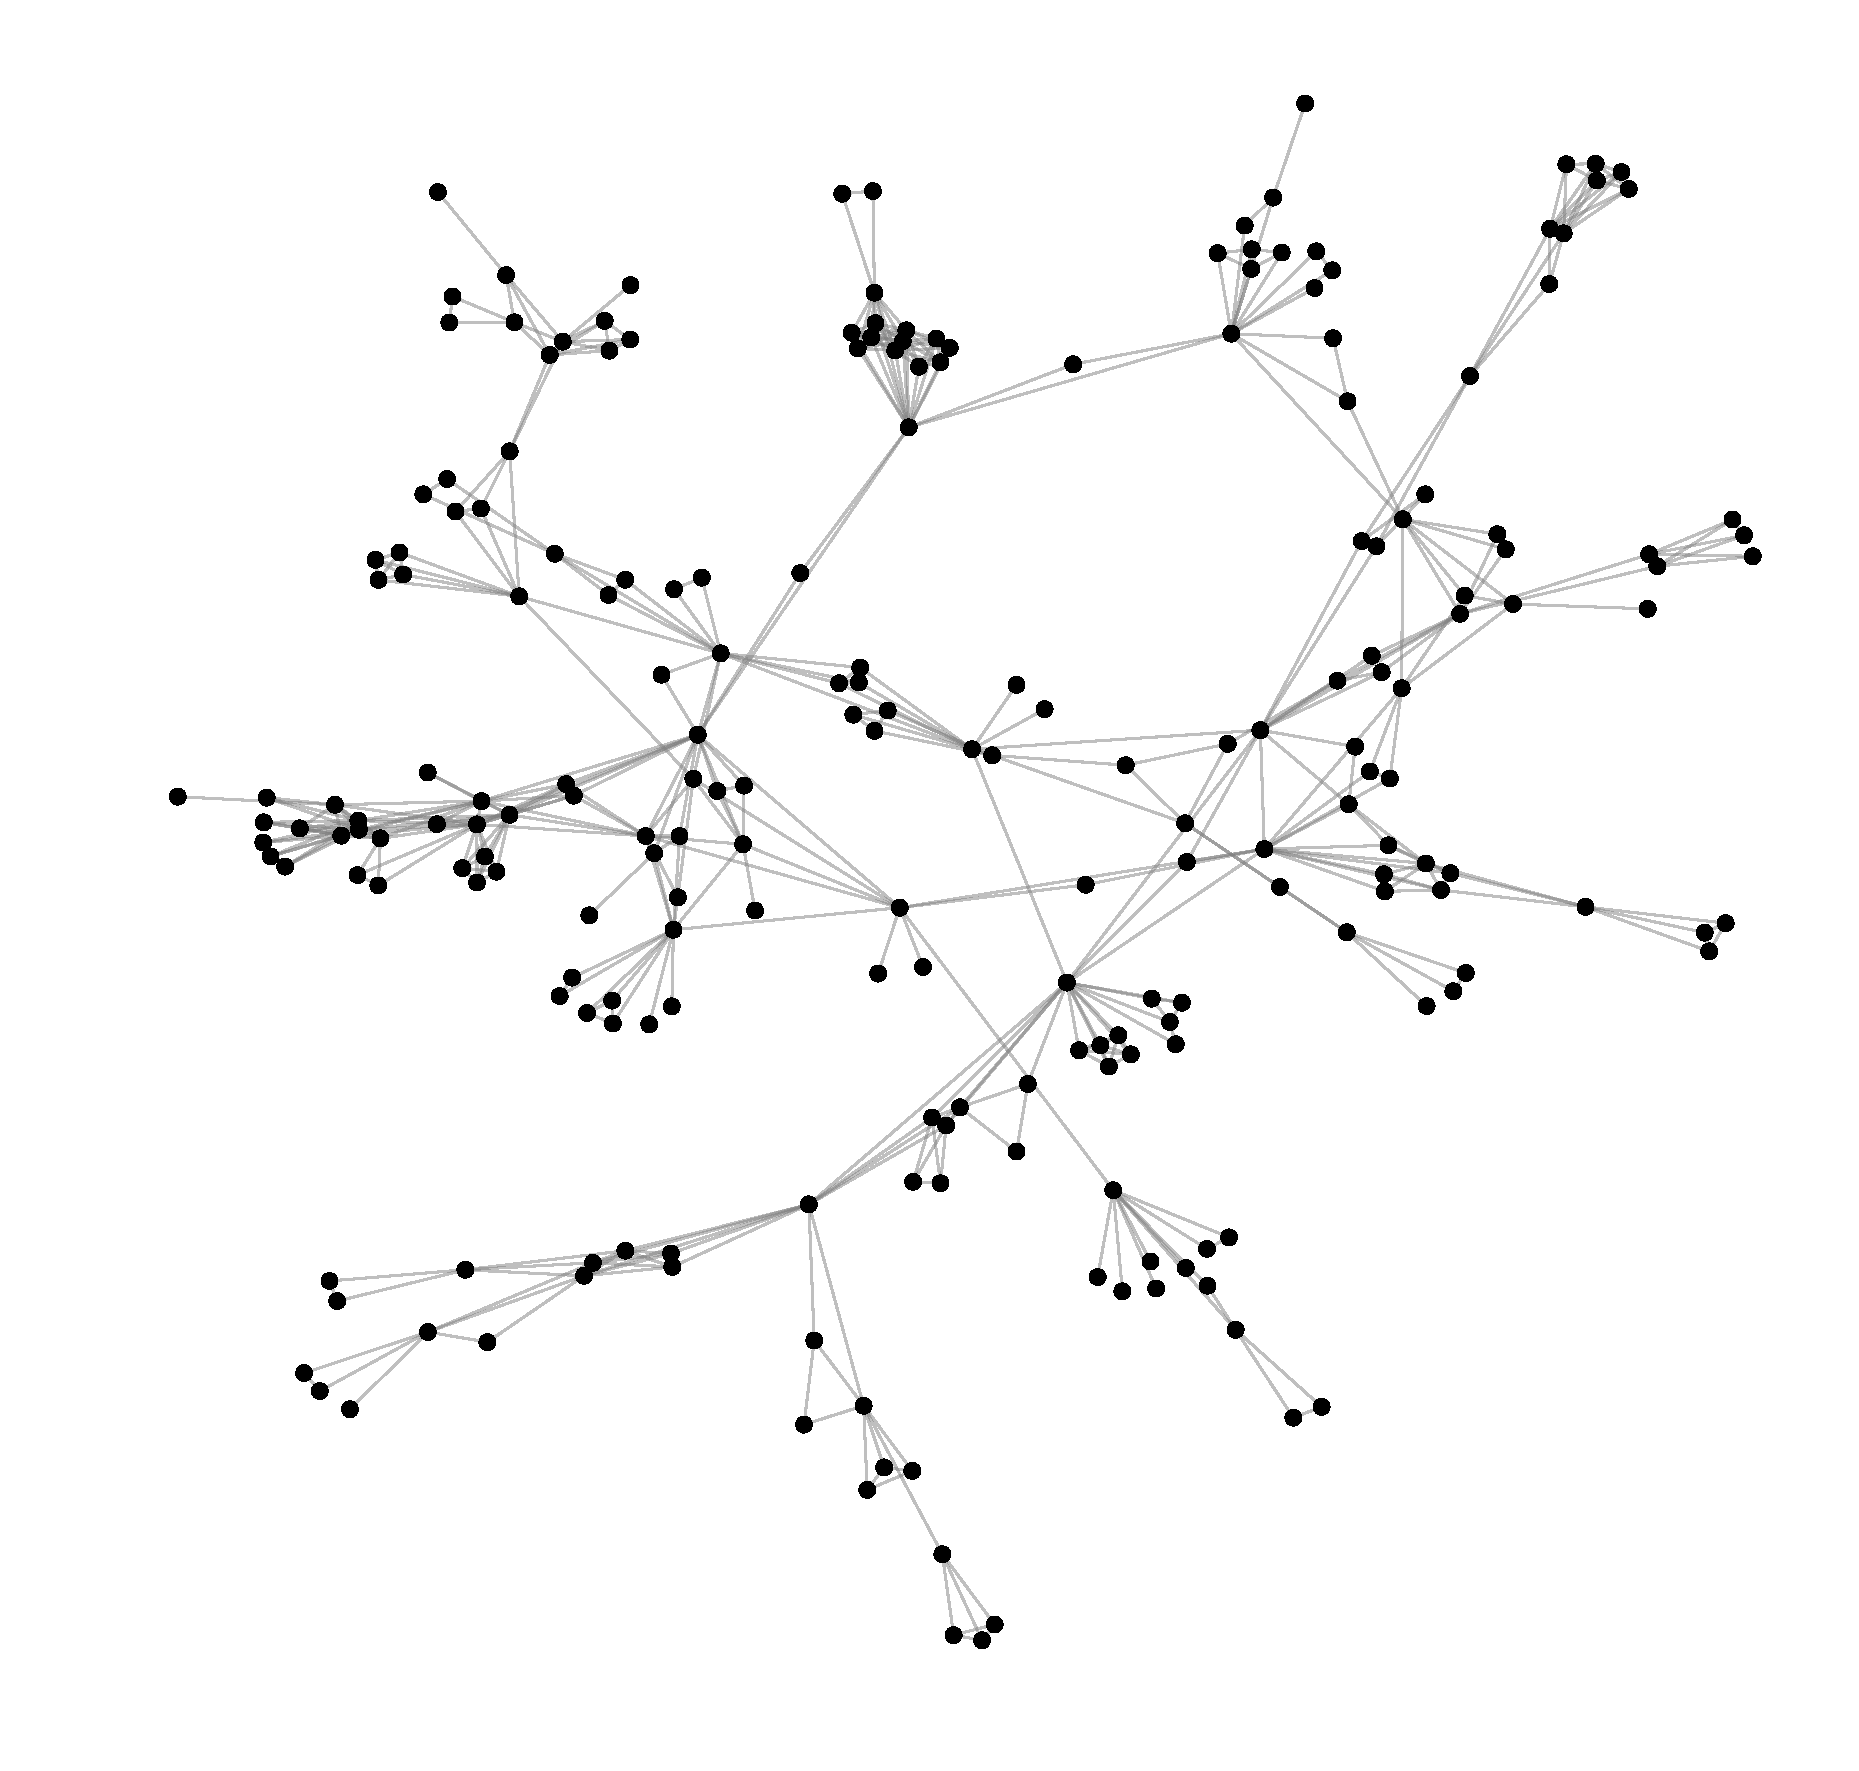
\includegraphics[width=.54\textwidth]{./assets/images/anarchy_network_cluster.pdf}
        \caption{\(G_3\) largest connected component,  \(\bar{G}_{3}\).}\label{fig:g_three_cluster}
     \end{subfigure}
     \caption{Graphical representations of \(G_1, G_2, G_3\) and their respective
     main clusters.}
\end{figure}

A summary of the collaborative metrics for all three co authorship networks is given by
Table~\ref{table:summary_other_networks} and the degree distribution of all three
networks is shown in Figure~\ref{fig:degree_distrs}.

\begin{table}[!hbtp]
    \centering
    \resizebox{\textwidth}{!}{
    \begin{tabular}{lrrrrrrrrrr}
\toprule
{} &  \# Nodes &  \# Edges &  \# Isolated nodes &  \% Isolated nodes &  \# Connected components &  Size of largest component &  Av. degree &  \# Communities &  Modularity &  Clustering coeff \\
\midrule
$G$              &     4221 &     7642 &               338 &               8.0 &                    1157 &                        796 &       3.621 &           1177 &    0.965264 &             0.666 \\
$\bar{G}$        &      796 &     2214 &                 0 &               0.0 &                       1 &                        796 &       5.563 &             29 &    0.840138 &             0.773 \\
Auction Games    &     5362 &     7861 &               453 &               8.4 &                    1469 &                       1348 &       2.932 &           1493 &    0.957238 &             0.599 \\
Price of Anarchy &     1315 &     1952 &               165 &              12.5 &                     406 &                        221 &       2.969 &            414 &    0.964498 &             0.626 \\
\bottomrule
\end{tabular}
}
    \caption{Network metrics for \(G_1, G_2, G_3\).}\label{table:summary_other_networks}
\end{table}

\begin{figure}[!hbtp]
    \centering
    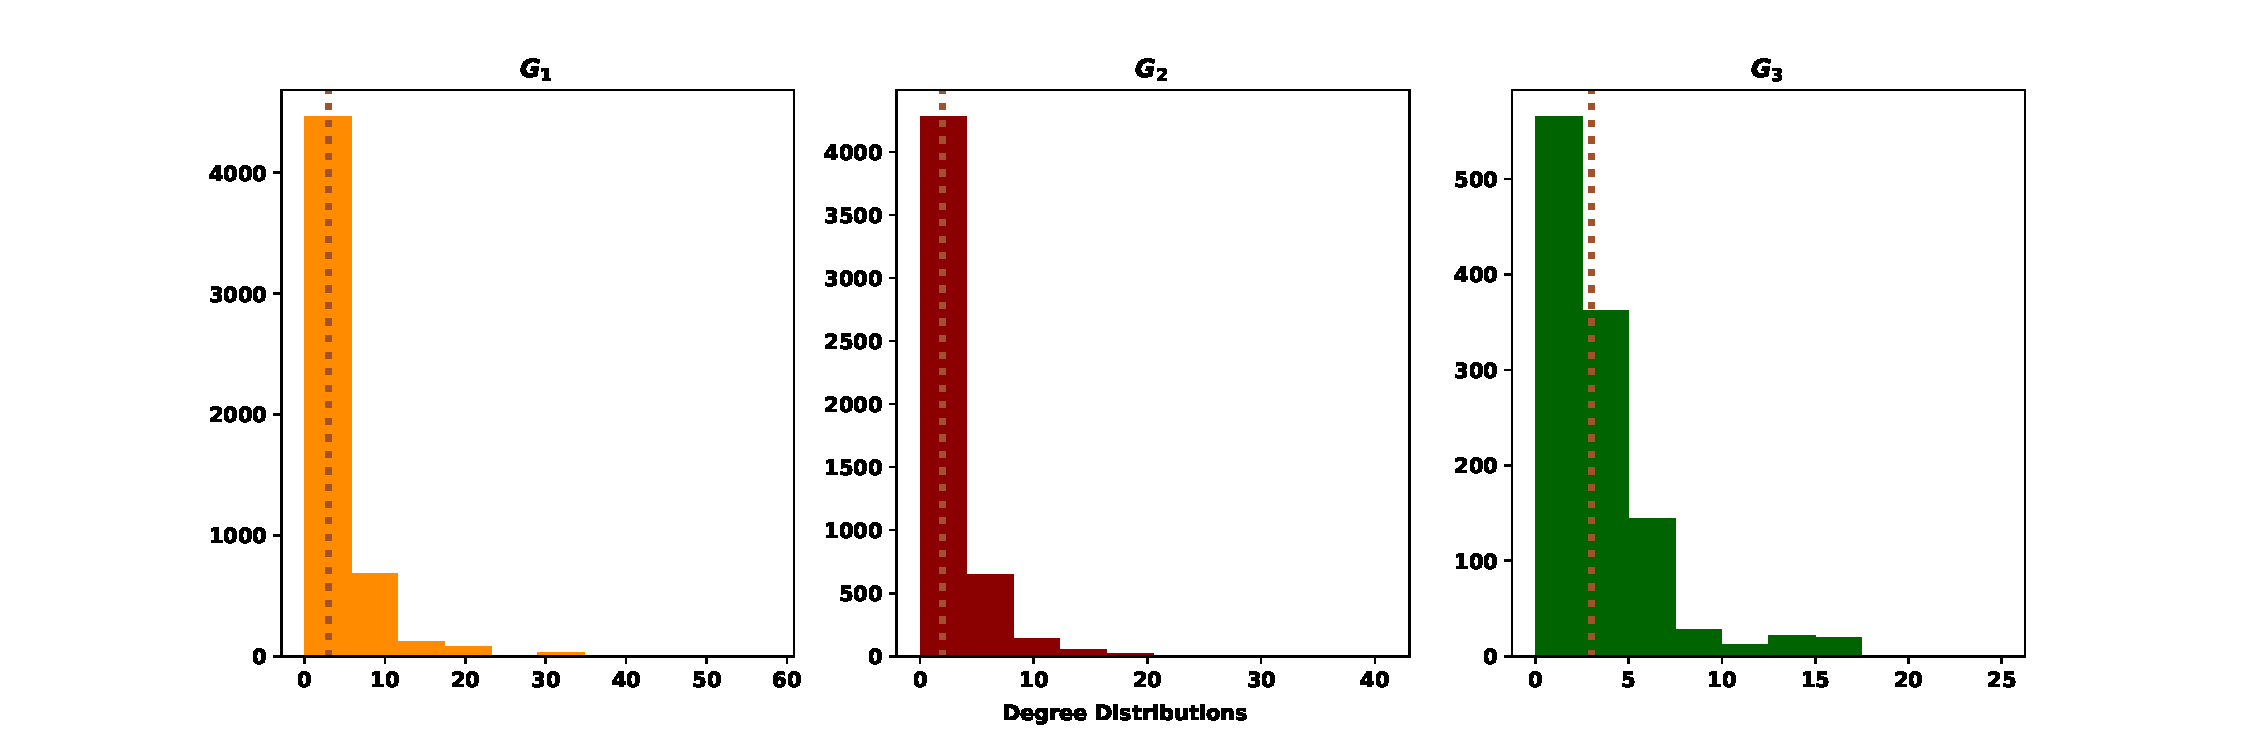
\includegraphics[width=\textwidth]{./assets/images/networks_ditributions.pdf}
    \caption{Degree distribution for networks \(G_1, G_2\) and \(G_3\). The descriptive
    statistics for each of the distribution are for \(G_1\): mean \(=3.85\),
    median \(=3\), std \(=4.25\). For \(G_2\): mean \(=3.04\), median \(=2\),
    std \(=3.01\) and for \(G_3\): mean \(=3.38\), median \(=3\), std \(=2.90\).
    It is clear that these distributions are not normally distributed, which has
    also been verified using a statistical test. Moreover, the statistical difference
    of the medians has been tested using a Kruskal Wallis test. The medians
    of \(G_1\) and \(G_3\) are not significantly different, however they are
    are significantly large than that of \(G_2\).}\label{fig:degree_distrs}
\end{figure}

Using Table~\ref{table:summary_other_networks} and Figure~\ref{fig:degree_distrs}
the following remarks can be made:

\begin{itemize}
    \item Comparing to another well studied topic, auction games, the field of the
    IPD appears to be more collaborative. Due to the
    value of the average degree, authors in \(G_1\) are known to have on average almost
    one more collaboration than \(G_2\). A slightly lower cluster coefficient ($ .622 < .702$)
    of auction games indicate that it is less likely for authors in \(G_2\) to collaborate
    with a co author.
    \item Regarding the price of anarchy, the measures indicate that the field
    is not as mature as the other two sub fields. There are no isolated authors,
    which is more of an indication of the time the field has been active. As a
    more recent field there had been better communication tools that enable more
    collaborations between researches. The average degree as well as the clustering
    coefficient (clustering coeff.$=0.713$) of \(G_3\) is comparable to those
    of the IPD.
\end{itemize}

These results can be extended to the main clusters of each network, as shown in
Table~\ref{table:summary_clusters}. The metrics' values are fairly similar and
the size of \(G_2\)'s main cluster does not appear to gave any significant
effect; all the same conclusions are made.

\begin{table}[!hbtp]
    \centering
    \resizebox{\textwidth}{!}{
    \begin{tabular}{lrrrrrrrrr}
\toprule
{} &  \# Nodes &  \# Edges &  \# Isolated nodes &  \% Isolated nodes &  \# Connected components &  Size of largest component &  Av. degree &  Modularity &  Clustering coeff \\
\midrule
Prisoner's Dilemma &      815 &     2300 &                 0 &               0.0 &                       1 &                        815 &       5.644 &       0.857 &             0.775 \\
Auction Games      &     1348 &     3158 &                 0 &               0.0 &                       1 &                       1348 &       4.685 &       0.858 &             0.699 \\
Price of Anarchy   &      221 &      520 &                 0 &               0.0 &                       1 &                        221 &       4.706 &       0.818 &             0.714 \\
\bottomrule
\end{tabular}
}
    \caption{Network metrics for largest components, \(\bar{G}_1, \bar{G}_2, \bar{G}_3\).}\label{table:summary_clusters}
\end{table}

The change of the networks over time is also studied by constructing the network
cumulatively using a year interval. A total of 64 sub graphs
over 64 periods, starting in 1950, were created and all the collaborative metrics
for each sub graph have been calculated. Note that years 1952 and 1953 have no
publications in our data set. The metrics of each network for each period are given by
Table~\ref{table:coll_cumulative}.
Similar to the results of~\cite{Liu2015}, it can been observed that the network \(G_1\)
grows over time and that the network always had a high value of modularity.

\begin{table}[!hbtp]
    \centering
    \begin{adjustbox}{totalheight=.8\textheight-2\baselineskip, width=\textwidth}
    \begin{tabular}{lrrrrrrrllr}
\toprule
{} &  \# Nodes &  \# Edges &  \# Isolated nodes &  \% Isolated nodes &  \# Connected components &  Size of largest component &  Av. degree & \# Communities & Modularity &  Clustering coeff \\
\midrule
1954 - 1950 &        3 &        0 &                 3 &             100.0 &                       3 &                          1 &       0.000 &             - &          - &             0.000 \\
1954 - 1955 &        2 &        0 &                 2 &             100.0 &                       2 &                          1 &       0.000 &             - &          - &             0.000 \\
1955 - 1956 &        3 &        0 &                 3 &             100.0 &                       3 &                          1 &       0.000 &             - &          - &             0.000 \\
1956 - 1957 &        4 &        0 &                 4 &             100.0 &                       4 &                          1 &       0.000 &             - &          - &             0.000 \\
1957 - 1958 &        6 &        0 &                 6 &             100.0 &                       6 &                          1 &       0.000 &             - &          - &             0.000 \\
1958 - 1959 &        7 &        0 &                 7 &             100.0 &                       7 &                          1 &       0.000 &             - &          - &             0.000 \\
1959 - 1961 &        7 &        0 &                 7 &             100.0 &                       7 &                          1 &       0.000 &             - &          - &             0.000 \\
1961 - 1962 &        8 &        0 &                 8 &             100.0 &                       8 &                          1 &       0.000 &             - &          - &             0.000 \\
1962 - 1964 &        9 &        0 &                 9 &             100.0 &                       9 &                          1 &       0.000 &             - &          - &             0.000 \\
1964 - 1965 &       10 &        0 &                10 &             100.0 &                      10 &                          1 &       0.000 &             - &          - &             0.000 \\
1965 - 1966 &       17 &        3 &                11 &              64.7 &                      14 &                          2 &       0.353 &            14 &   0.666667 &             0.000 \\
1966 - 1967 &       21 &        4 &                13 &              61.9 &                      17 &                          2 &       0.381 &            17 &       0.75 &             0.000 \\
1967 - 1968 &       32 &       15 &                13 &              40.6 &                      21 &                          5 &       0.938 &            21 &   0.684444 &             0.135 \\
1968 - 1969 &       36 &       17 &                16 &              44.4 &                      24 &                          6 &       0.944 &            24 &   0.629758 &             0.139 \\
1969 - 1970 &       39 &       18 &                17 &              43.6 &                      26 &                          6 &       0.923 &            26 &   0.666667 &             0.128 \\
1970 - 1971 &       51 &       28 &                18 &              35.3 &                      31 &                          6 &       1.098 &            31 &   0.826531 &             0.275 \\
1971 - 1972 &       58 &       34 &                19 &              32.8 &                      34 &                          6 &       1.172 &            34 &   0.866782 &             0.345 \\
1972 - 1973 &       59 &       35 &                18 &              30.5 &                      34 &                          6 &       1.186 &            34 &   0.873469 &             0.339 \\
1973 - 1974 &       59 &       35 &                18 &              30.5 &                      34 &                          6 &       1.186 &            34 &   0.873469 &             0.339 \\
1974 - 1975 &       60 &       35 &                19 &              31.7 &                      35 &                          6 &       1.167 &            35 &   0.873469 &             0.333 \\
1975 - 1976 &       60 &       35 &                19 &              31.7 &                      35 &                          6 &       1.167 &            35 &   0.873469 &             0.333 \\
1976 - 1977 &       68 &       37 &                23 &              33.8 &                      41 &                          6 &       1.088 &            41 &   0.885318 &             0.294 \\
1977 - 1978 &       70 &       38 &                23 &              32.9 &                      42 &                          6 &       1.086 &            42 &   0.890582 &             0.286 \\
1978 - 1979 &       73 &       42 &                23 &              31.5 &                      42 &                          6 &       1.151 &            42 &   0.893424 &             0.292 \\
1979 - 1980 &       77 &       45 &                25 &              32.5 &                      44 &                          6 &       1.169 &            44 &   0.899753 &             0.307 \\
1980 - 1981 &       80 &       50 &                26 &              32.5 &                      45 &                          6 &       1.250 &            45 &     0.8928 &             0.318 \\
1981 - 1982 &       84 &       56 &                26 &              31.0 &                      46 &                          6 &       1.333 &            46 &   0.903061 &             0.350 \\
1982 - 1983 &       87 &       57 &                27 &              31.0 &                      48 &                          6 &       1.310 &            48 &   0.906125 &             0.338 \\
1983 - 1984 &       94 &       58 &                32 &              34.0 &                      54 &                          6 &       1.234 &            54 &   0.909037 &             0.313 \\
1984 - 1985 &       95 &       58 &                33 &              34.7 &                      55 &                          6 &       1.221 &            55 &   0.909037 &             0.309 \\
1985 - 1986 &      104 &       59 &                40 &              38.5 &                      63 &                          6 &       1.135 &            63 &   0.911807 &             0.283 \\
1986 - 1987 &      116 &       61 &                48 &              41.4 &                      73 &                          6 &       1.052 &            73 &   0.916958 &             0.253 \\
1987 - 1988 &      121 &       65 &                48 &              39.7 &                      75 &                          6 &       1.074 &            75 &   0.924497 &             0.268 \\
1988 - 1989 &      134 &       76 &                47 &              35.1 &                      80 &                          6 &       1.134 &            80 &   0.937673 &             0.272 \\
1989 - 1990 &      145 &       82 &                49 &              33.8 &                      86 &                          6 &       1.131 &            86 &   0.944676 &             0.272 \\
1990 - 1991 &      158 &       88 &                53 &              33.5 &                      94 &                          6 &       1.114 &            94 &   0.950413 &             0.268 \\
1991 - 1992 &      169 &       91 &                59 &              34.9 &                     102 &                          6 &       1.077 &           102 &   0.953025 &             0.251 \\
1992 - 1993 &      186 &      104 &                62 &              33.3 &                     110 &                          6 &       1.118 &           110 &    0.95932 &             0.266 \\
1993 - 1994 &      220 &      134 &                72 &              32.7 &                     127 &                          6 &       1.218 &           127 &   0.965471 &             0.317 \\
1994 - 1995 &      239 &      144 &                74 &              31.0 &                     137 &                          6 &       1.205 &           137 &   0.969329 &             0.304 \\
1995 - 1996 &      257 &      163 &                77 &              30.0 &                     145 &                          6 &       1.268 &           145 &   0.970831 &             0.318 \\
1996 - 1997 &      279 &      178 &                81 &              29.0 &                     156 &                          6 &       1.276 &           156 &   0.974309 &             0.336 \\
1997 - 1998 &      311 &      215 &                65 &              20.9 &                     160 &                          6 &       1.383 &           160 &   0.979773 &             0.354 \\
1998 - 1999 &      329 &      239 &                58 &              17.6 &                     162 &                          6 &       1.453 &           162 &   0.981741 &             0.376 \\
1999 - 2000 &      373 &      273 &                67 &              18.0 &                     183 &                          6 &       1.464 &           183 &   0.983778 &             0.387 \\
2000 - 2001 &      400 &      320 &                54 &              13.5 &                     184 &                          7 &       1.600 &           184 &   0.983066 &             0.410 \\
2001 - 2002 &      450 &      366 &                61 &              13.6 &                     206 &                          7 &       1.627 &           206 &   0.984547 &             0.418 \\
2002 - 2003 &      509 &      414 &                58 &              11.4 &                     229 &                          7 &       1.627 &           229 &   0.987083 &             0.421 \\
2003 - 2004 &      580 &      489 &                58 &              10.0 &                     253 &                         10 &       1.686 &           253 &   0.988052 &             0.429 \\
2004 - 2005 &      679 &      599 &                57 &               8.4 &                     284 &                         19 &       1.764 &           284 &    0.98891 &             0.463 \\
2005 - 2006 &      854 &      806 &                66 &               7.7 &                     342 &                         21 &       1.888 &           342 &   0.990724 &             0.496 \\
2006 - 2007 &     1056 &     1117 &                76 &               7.2 &                     402 &                         24 &       2.116 &           402 &   0.989663 &             0.527 \\
2007 - 2008 &     1255 &     1460 &                85 &               6.8 &                     454 &                         32 &       2.327 &           455 &   0.989753 &             0.549 \\
2008 - 2009 &     1462 &     1759 &               104 &               7.1 &                     520 &                         56 &       2.406 &           521 &   0.987517 &             0.550 \\
2009 - 2010 &     1700 &     2301 &               114 &               6.7 &                     581 &                         99 &       2.707 &           584 &   0.979084 &             0.571 \\
2010 - 2011 &     2040 &     2954 &               121 &               5.9 &                     665 &                        121 &       2.896 &           668 &   0.980477 &             0.603 \\
2011 - 2012 &     2422 &     3676 &               126 &               5.2 &                     756 &                        210 &       3.036 &           759 &   0.979196 &             0.629 \\
2012 - 2013 &     2807 &     4398 &               138 &               4.9 &                     843 &                        330 &       3.134 &           849 &   0.976132 &             0.639 \\
2013 - 2014 &     3199 &     5044 &               148 &               4.6 &                     942 &                        406 &       3.153 &           950 &   0.974968 &             0.651 \\
2014 - 2015 &     3798 &     6221 &               159 &               4.2 &                    1064 &                        514 &       3.276 &          1074 &   0.976242 &             0.668 \\
2015 - 2016 &     4472 &     8344 &               169 &               3.8 &                    1184 &                        614 &       3.732 &          1198 &   0.975233 &             0.690 \\
2016 - 2017 &     4925 &     9235 &               173 &               3.5 &                    1274 &                        703 &       3.750 &          1292 &   0.976353 &             0.700 \\
2017 - 2018 &     5385 &    10379 &               176 &               3.3 &                    1356 &                        815 &       3.855 &          1369 &   0.977318 &             0.708 \\
\bottomrule
\end{tabular}
}
    \caption{Collaborativeness metrics for cumulative graphs, \(G \subseteq G_1\).}\label{table:coll_cumulative}
\end{adjustbox}
\end{table}

\begin{table}[!hbtp]
    \centering
    \begin{adjustbox}{totalheight=\textheight-2\baselineskip, width=\textwidth}
    \begin{tabular}{lrrrrrrrrrr}
\toprule
Periods &  \# Nodes &  \# Edges &  \# Isolated nodes &  \% Isolated nodes &  \# Connected components &  Size of largest component &  Av. degree &  \# Communities &  Modularity &  Clustering coeff \\
\midrule
1951 - 1966 &        2 &        1 &                 0 &               0.0 &                       1 &                          2 &       1.000 &              1 &       0.000 &             0.000 \\
1951 - 1967 &        2 &        1 &                 0 &               0.0 &                       1 &                          2 &       1.000 &              1 &       0.000 &             0.000 \\
1951 - 1968 &        5 &        8 &                 0 &               0.0 &                       1 &                          5 &       3.200 &              1 &       0.000 &             0.867 \\
1951 - 1969 &        6 &       10 &                 0 &               0.0 &                       1 &                          6 &       3.333 &              2 &       0.020 &             0.833 \\
1951 - 1970 &        6 &       10 &                 0 &               0.0 &                       1 &                          6 &       3.333 &              2 &       0.020 &             0.833 \\
1951 - 1971 &        6 &       10 &                 0 &               0.0 &                       1 &                          6 &       3.333 &              2 &       0.020 &             0.833 \\
1951 - 1972 &        6 &       10 &                 0 &               0.0 &                       1 &                          6 &       3.333 &              2 &       0.020 &             0.833 \\
1951 - 1973 &        6 &       10 &                 0 &               0.0 &                       1 &                          6 &       3.333 &              2 &       0.020 &             0.833 \\
1951 - 1974 &        6 &       10 &                 0 &               0.0 &                       1 &                          6 &       3.333 &              2 &       0.020 &             0.833 \\
1951 - 1976 &        6 &       10 &                 0 &               0.0 &                       1 &                          6 &       3.333 &              2 &       0.020 &             0.833 \\
1951 - 1977 &        6 &       10 &                 0 &               0.0 &                       1 &                          6 &       3.333 &              2 &       0.020 &             0.833 \\
1951 - 1978 &        6 &       10 &                 0 &               0.0 &                       1 &                          6 &       3.333 &              2 &       0.020 &             0.833 \\
1951 - 1979 &        6 &       10 &                 0 &               0.0 &                       1 &                          6 &       3.333 &              2 &       0.020 &             0.833 \\
1951 - 1980 &        6 &       10 &                 0 &               0.0 &                       1 &                          6 &       3.333 &              2 &       0.020 &             0.833 \\
1951 - 1981 &        6 &       10 &                 0 &               0.0 &                       1 &                          6 &       3.333 &              2 &       0.020 &             0.833 \\
1951 - 1983 &        6 &       10 &                 0 &               0.0 &                       1 &                          6 &       3.333 &              2 &       0.020 &             0.833 \\
1951 - 1984 &        6 &       10 &                 0 &               0.0 &                       1 &                          6 &       3.333 &              2 &       0.020 &             0.833 \\
1951 - 1985 &        6 &       10 &                 0 &               0.0 &                       1 &                          6 &       3.333 &              2 &       0.020 &             0.833 \\
1951 - 1986 &        6 &       10 &                 0 &               0.0 &                       1 &                          6 &       3.333 &              2 &       0.020 &             0.833 \\
1951 - 1987 &        6 &       10 &                 0 &               0.0 &                       1 &                          6 &       3.333 &              2 &       0.020 &             0.833 \\
1951 - 1988 &        6 &       10 &                 0 &               0.0 &                       1 &                          6 &       3.333 &              2 &       0.020 &             0.833 \\
1951 - 1989 &        6 &       10 &                 0 &               0.0 &                       1 &                          6 &       3.333 &              2 &       0.020 &             0.833 \\
1951 - 1990 &        6 &       10 &                 0 &               0.0 &                       1 &                          6 &       3.333 &              2 &       0.020 &             0.833 \\
1951 - 1991 &        6 &       10 &                 0 &               0.0 &                       1 &                          6 &       3.333 &              2 &       0.020 &             0.833 \\
1951 - 1992 &        6 &       10 &                 0 &               0.0 &                       1 &                          6 &       3.333 &              2 &       0.020 &             0.833 \\
1951 - 1993 &        6 &       10 &                 0 &               0.0 &                       1 &                          6 &       3.333 &              2 &       0.020 &             0.833 \\
1951 - 1994 &        6 &       10 &                 0 &               0.0 &                       1 &                          6 &       3.333 &              2 &       0.020 &             0.833 \\
1951 - 1995 &        6 &       10 &                 0 &               0.0 &                       1 &                          6 &       3.333 &              2 &       0.020 &             0.833 \\
1951 - 1996 &        6 &       10 &                 0 &               0.0 &                       1 &                          6 &       3.333 &              2 &       0.020 &             0.833 \\
1951 - 1997 &        6 &       10 &                 0 &               0.0 &                       1 &                          6 &       3.333 &              2 &       0.020 &             0.833 \\
1951 - 1998 &        6 &       10 &                 0 &               0.0 &                       1 &                          6 &       3.333 &              2 &       0.020 &             0.833 \\
1951 - 1999 &        6 &       10 &                 0 &               0.0 &                       1 &                          6 &       3.333 &              2 &       0.020 &             0.833 \\
1951 - 2000 &        6 &       10 &                 0 &               0.0 &                       1 &                          6 &       3.333 &              2 &       0.020 &             0.833 \\
1951 - 2001 &        7 &       21 &                 0 &               0.0 &                       1 &                          7 &       6.000 &              1 &       0.000 &             1.000 \\
1951 - 2002 &        7 &       21 &                 0 &               0.0 &                       1 &                          7 &       6.000 &              1 &       0.000 &             1.000 \\
1951 - 2003 &        7 &       21 &                 0 &               0.0 &                       1 &                          7 &       6.000 &              1 &       0.000 &             1.000 \\
1951 - 2004 &       10 &       13 &                 0 &               0.0 &                       1 &                         10 &       2.600 &              2 &       0.376 &             0.553 \\
1951 - 2005 &       19 &       28 &                 0 &               0.0 &                       1 &                         19 &       2.947 &              3 &       0.544 &             0.730 \\
1951 - 2006 &       22 &       35 &                 0 &               0.0 &                       1 &                         22 &       3.182 &              4 &       0.527 &             0.720 \\
1951 - 2007 &       25 &       39 &                 0 &               0.0 &                       1 &                         25 &       3.120 &              5 &       0.558 &             0.686 \\
1951 - 2008 &       33 &       62 &                 0 &               0.0 &                       1 &                         33 &       3.758 &              4 &       0.623 &             0.736 \\
1951 - 2009 &       71 &      148 &                 0 &               0.0 &                       1 &                         71 &       4.169 &              6 &       0.697 &             0.698 \\
1951 - 2010 &      133 &      387 &                 0 &               0.0 &                       1 &                        133 &       5.820 &              7 &       0.726 &             0.749 \\
1951 - 2011 &      157 &      465 &                 0 &               0.0 &                       1 &                        157 &       5.924 &              8 &       0.727 &             0.725 \\
1951 - 2012 &      209 &      611 &                 0 &               0.0 &                       1 &                        209 &       5.847 &             11 &       0.733 &             0.737 \\
1951 - 2013 &      322 &      892 &                 0 &               0.0 &                       1 &                        322 &       5.540 &             12 &       0.780 &             0.743 \\
1951 - 2014 &      399 &     1109 &                 0 &               0.0 &                       1 &                        399 &       5.559 &             15 &       0.794 &             0.742 \\
1951 - 2015 &      504 &     1368 &                 0 &               0.0 &                       1 &                        504 &       5.429 &             24 &       0.811 &             0.751 \\
1951 - 2016 &      613 &     1677 &                 0 &               0.0 &                       1 &                        613 &       5.471 &             21 &       0.819 &             0.761 \\
1951 - 2017 &      706 &     1935 &                 0 &               0.0 &                       1 &                        706 &       5.482 &             29 &       0.830 &             0.772 \\
1951 - 2018 &      796 &     2214 &                 0 &               0.0 &                       1 &                        796 &       5.563 &             25 &       0.845 &             0.773 \\
\bottomrule
\end{tabular}
}
    \caption{Collaborativeness metrics for cumulative graphs' main clusters, \(G \subseteq \bar{G}_1\).}\label{table:clusters_cumulative}
\end{adjustbox}
\end{table}

To better assess the change over time for each metric they have been plotted in
Figure~\ref{fig:cumulative_networks}. The number of nodes, connected components
and the size of largest component have been normalised such that the trend between
the three networks can be compared.

\begin{itemize}
    \item In Figure~\ref{fig:normalised_number_nodes} the normalised number of nodes,
    which is calculated by dividing by the total number of nodes in each respective network,
    is shown. A steep increase in the size of all three networks is spotted soon after
    2000. This could indicate that more data have been available in the sources
    used in this work following the year 2000. It is however, definitely not a effect
    of a single field, as it is true for all three sub fields considered here.
    The sudden increase following the year 2000, is also reported by the
    number of connected components and the size of the main cluster, Figures
    \ref{fig:normalised_number_connected_components}, \ref{fig:normalised_size_of_cc}.
    A connected components represents at least one publication which means that indeed
    more articles are being gathered from 2000 onwards.
    \item Auction games have been throughout of time less collaborative compared
    to the IPD. The average degree (Figure~\ref{fig:average_degree})
    and the clustering coefficient (Figure~\ref{fig:clustering_coefficient}) of 
    the cumulative sub graphs have been lower than that of \(G_1\).
    The only exception is during the years 2001-2008. For these
    year auction games appear to have had a more collaborative environment.
    \item In the price of anarchy cumulative graphs a sharp increase since the 
    beginning of the field can be observed for all metrics. There are not
    many data points due to the recent development of the field, however
    these steep trends could be an indication that game theoretic and potentially
    all scientific research has over time been more collaborative. This could
    be due to logistic and technical solutions.
    \item The high values of modularity throughout time is not true only for the
    network reported in~\cite{Liu2015} but also for all three networks of this
    field. Indicating that authors tend to create communities and write only
    with people from their communities and not others.
\end{itemize}

\begin{figure}[!hbtp]
    \centering
    \begin{subfigure}{.45\textwidth}\centering
        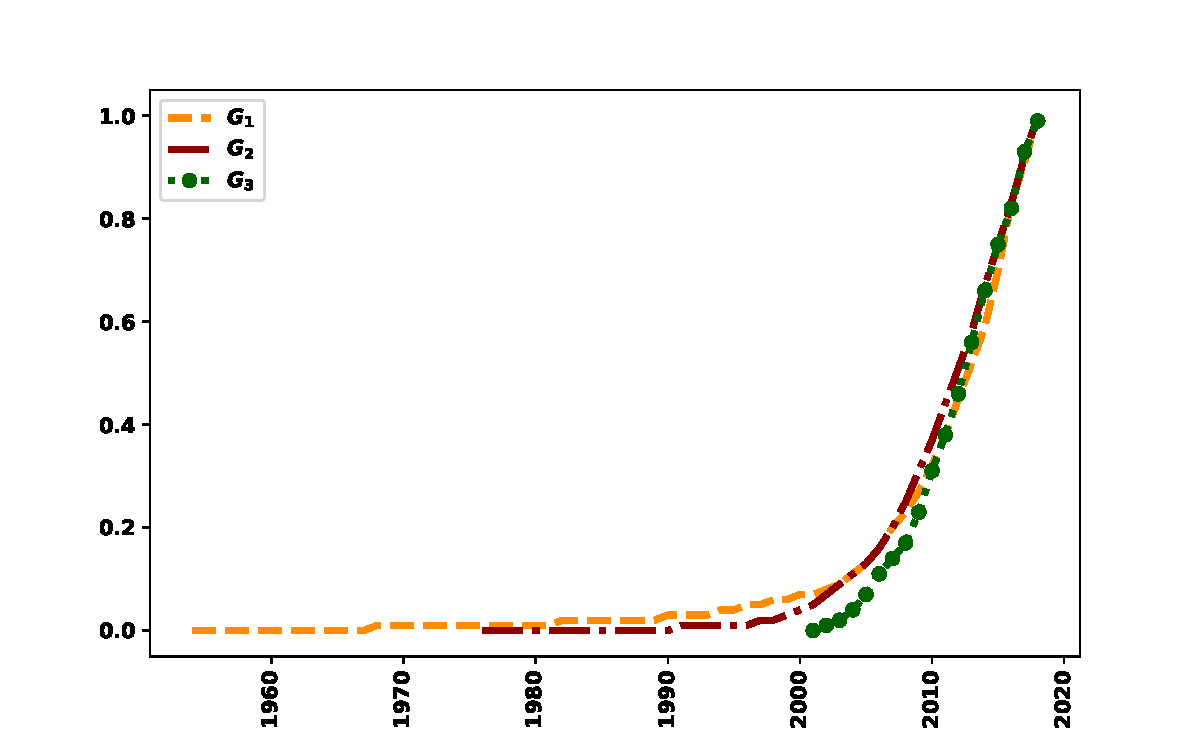
\includegraphics[width=1.1\textwidth]{./assets/images/percentage_networks_nodes.pdf}
        \caption{\% Nodes.}\label{fig:normalised_number_nodes}
    \end{subfigure}
    \begin{subfigure}{.45\textwidth}\centering
        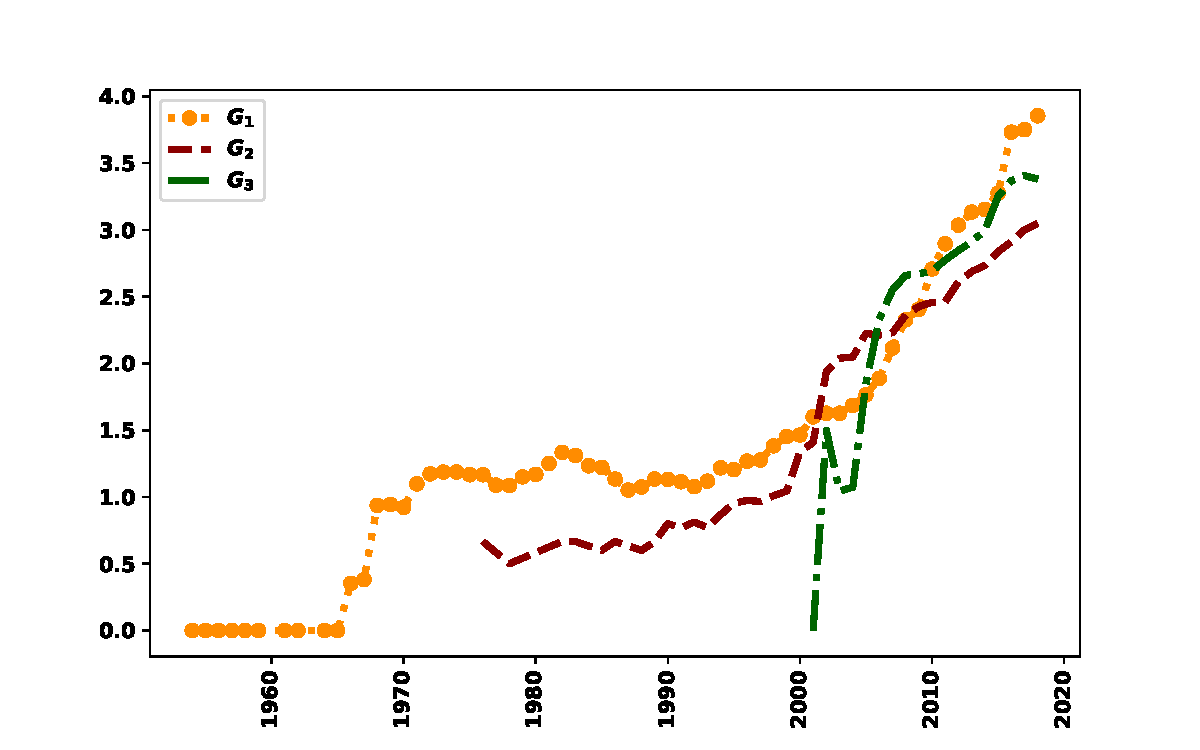
\includegraphics[width=1.1\textwidth]{./assets/images/degrees_over_time.pdf}
        \caption{Average Degree.}\label{fig:average_degree}
     \end{subfigure}

     \begin{subfigure}{.45\textwidth}\centering
        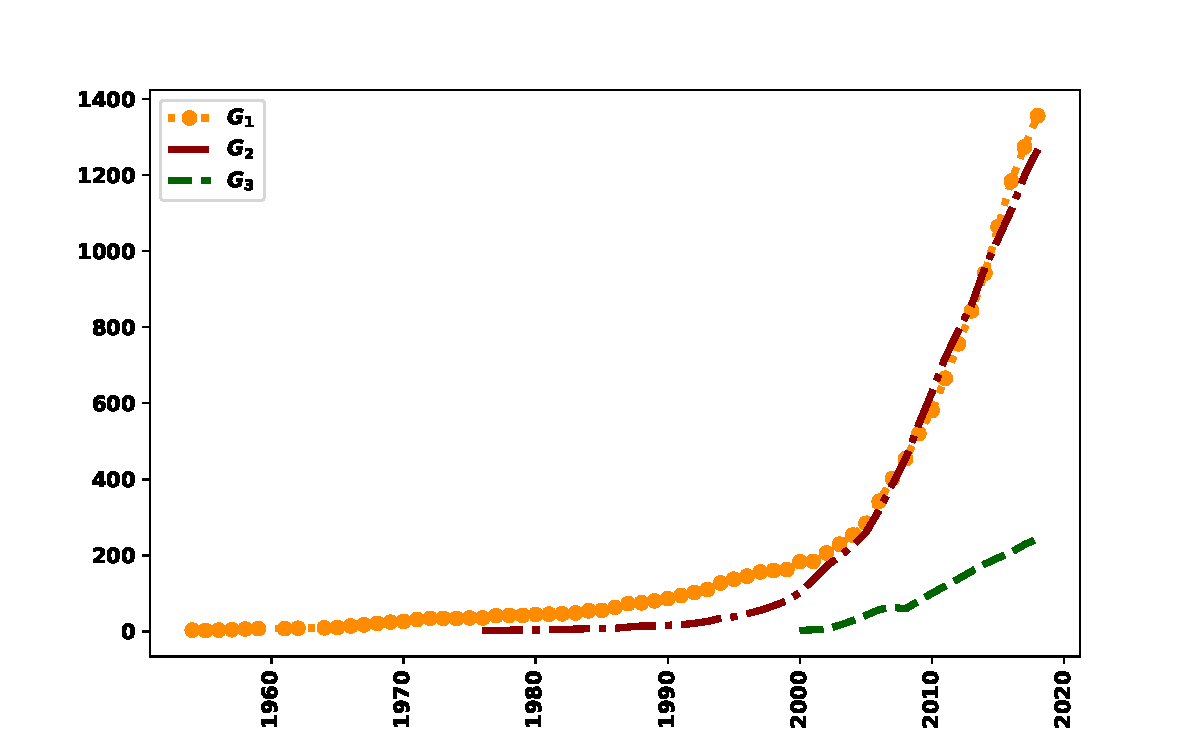
\includegraphics[width=1.1\textwidth]{./assets/images/connected_components_over_time.pdf}
        \caption{\% Connected components.}\label{fig:normalised_number_connected_components}
     \end{subfigure}
    \begin{subfigure}{.45\textwidth}\centering
        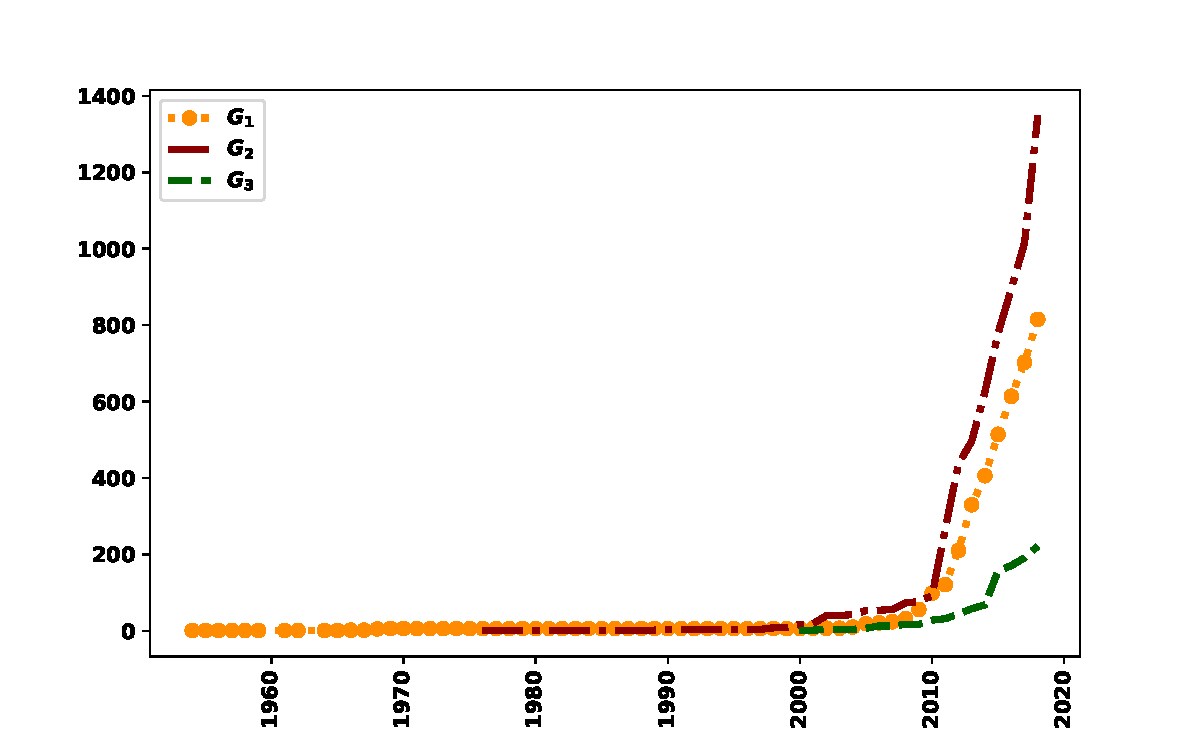
\includegraphics[width=1.1\textwidth]{./assets/images/size_of_largest_cc_over_time.pdf}
        \caption{\% Size of largest connected component.}\label{fig:normalised_size_of_cc}
    \end{subfigure}

    \begin{subfigure}{.45\textwidth}\centering
        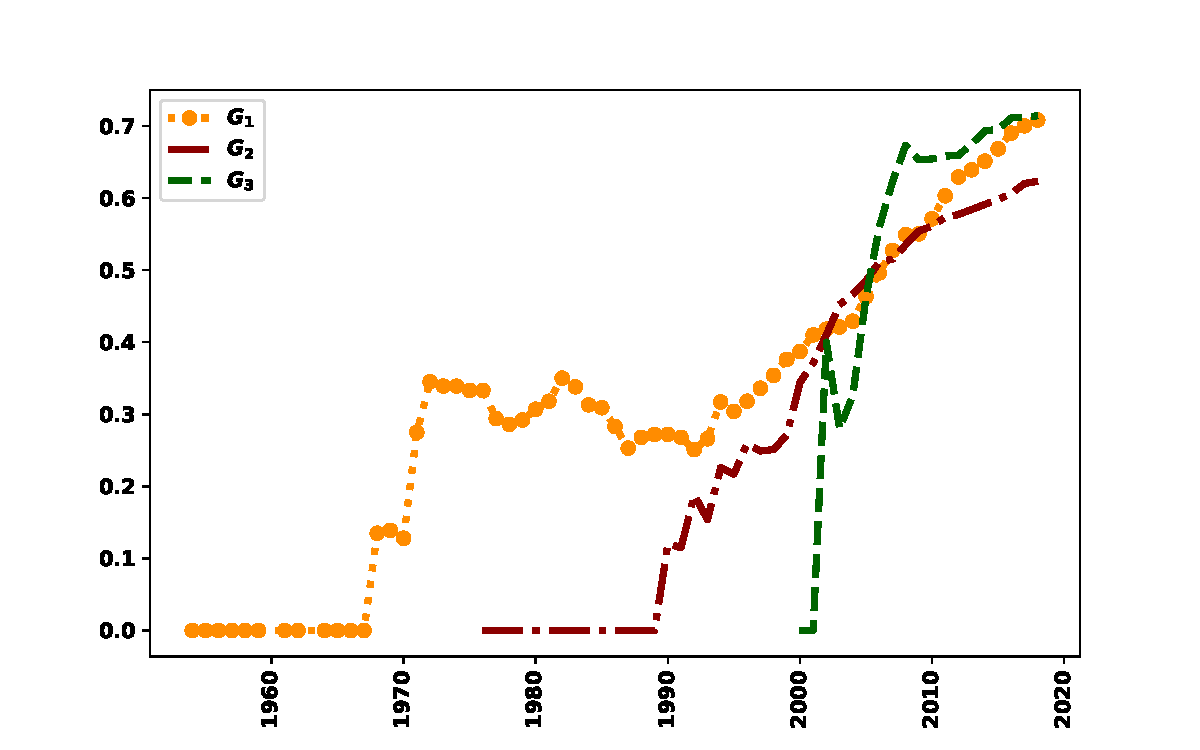
\includegraphics[width=1.1\textwidth]{./assets/images/clustering_coeff_over_time.pdf}
        \caption{Clustering coefficient.}\label{fig:clustering_coefficient}
     \end{subfigure}
     \begin{subfigure}{.45\textwidth}\centering
        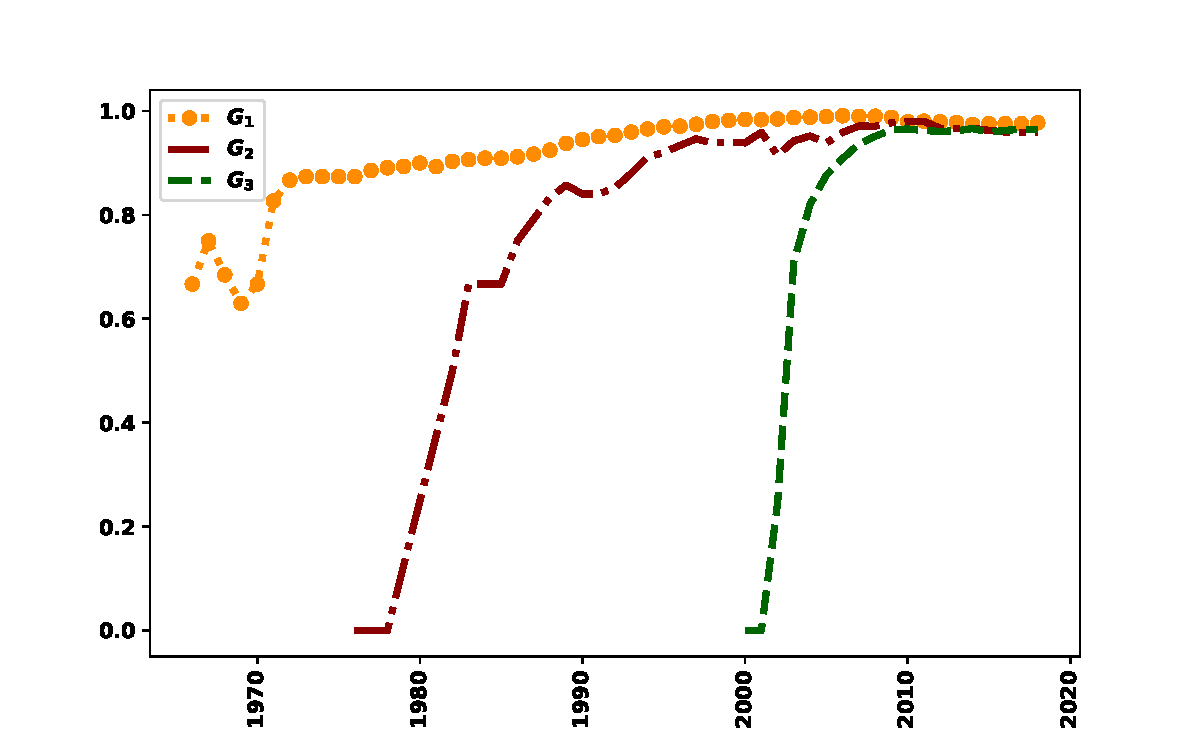
\includegraphics[width=1.1\textwidth]{./assets/images/modularity_over_time.pdf}
        \caption{Modularity.}\label{fig:modularity}
     \end{subfigure}
    \caption{Collaborative metrics over time for cumulative networks for \(G_1\),
    \(G_2\) and \(G_3\).}\label{fig:cumulative_networks}
\end{figure}

The cumulative collaborative metrics have also been calculated for each main
cluster, given in Table~\ref{table:clusters_cumulative}. Similarly, the results
do not appear to change over the main cluster.

The next results discussed here are on centrality measures. As a reminder,
two centrality measures are reported here, these are the closeness centrality
and the betweenness centrality. Closeness centrality is a measure of how
easy is for an author to contact others, and consequently affect them; influence them.
Thus closeness centrality here is a measure of influence. Betweenness centrality
is a measure of how many paths pass through a specific node, thus the amount
of information this person has access to. Betweenness centrality is used here
as a measure of how much an author gain from the field. All centrality measure
can have values ranging from \([0, 1]\).

For \(G_1\)
the most central author based on closeness and betweenness are given by Tables
\ref{table:central_authors_cc} and \ref{table:central_authors} respectively.
The betweenness centrality of the
most central authors in \(G_1\) are rather low with the highest ranked author
being Matjaz Perc with a between centrality of 0.008, Table~\ref{table:central_authors}.
A publication of Perc's work has been briefly discussed in
Section, and the centrality measure suggest that the network is influenced by him.
He is connected to a total of 58 nodes and he has published to all five of the different
sources considered in the study. Though he also gains from his position
in the network, the gain is minor. An author who is not in the top influencers but
does indeed gain from his position in the network is Martin Nowak, who was
extensively discussed in Section~\ref{section:timeline}.

\begin{figure}[H]
    \centering
    \begin{minipage}{.45\textwidth}
        \centering
        \begin{tabular}{llr}
\toprule
{} &             Name &  Closeness \\
\midrule
1  &      Matjaz Perc &   0.061854 \\
2  &     Yamir Moreno &   0.057163 \\
3  &        Long Wang &   0.056003 \\
4  &        Zhen Wang &   0.055938 \\
5  &  Attila Szolnoki &   0.055367 \\
6  &    Luo-Luo Jiang &   0.053405 \\
7  &    Arne Traulsen &   0.053153 \\
8  &     Cheng-Yi Xia &   0.052018 \\
9  &  Valerio Capraro &   0.051651 \\
10 &    Angel Sanchez &   0.051523 \\
\bottomrule
\end{tabular}

        \caption{Ten most influenced authors in \(G_1\).}\label{table:central_authors_cc}
    \end{minipage}%
    \begin{minipage}{.45\textwidth}
        \centering
        \begin{tabular}{llr}
\toprule
{} &       Name &  Betweeness \\
\midrule
1  &    M. Perc &    0.018903 \\
2  &    Z. Wang &    0.015962 \\
3  &    L. Wang &    0.014842 \\
4  &   Y. Zhang &    0.013178 \\
5  &   M. Nowak &    0.011588 \\
6  &    H. Wang &    0.008221 \\
7  &    Y. Chen &    0.008070 \\
8  &      Y. Li &    0.007993 \\
9  &  Y. Moreno &    0.007132 \\
10 &  N. Masuda &    0.006087 \\
\bottomrule
\end{tabular}

        \caption{Authors that gain the most influence in \(G_1\).}\label{table:central_authors}
    \end{minipage}
\end{figure}

From Tables~\ref{table:central_authors_cc} and \ref{table:central_authors} it
can be seen that authors in \(G_1\) are more likely to affect their field instead
of gaining from it. This can be better explored by considering the distributions
of the centralities and by comparing them to other fields.
The distributions for both centralities are
plotted in Figures~\ref{fig:betweenness_dist} and~\ref{fig:closeness_dist}, and
in Figures~\ref{fig:betweenness_dist_cluster} and~\ref{fig:closeness_dist_cluster}
for their respective main clusters.

Regarding gaining from your network. An author is more likely to gain more
from the influence of the field if they were authors in auction games or the
price of anarchy. Though if it were an author in the main cluster it would make
no statistical difference in which field they were to published. Overall,
all the betweenness values are rather small and the distributions skewed to the
left. This could imply that in all three networks, authors do not gain much from
the influence of their fields.

\begin{figure}[!hbtp]
    \centering
    \begin{subfigure}{\textwidth}\centering
        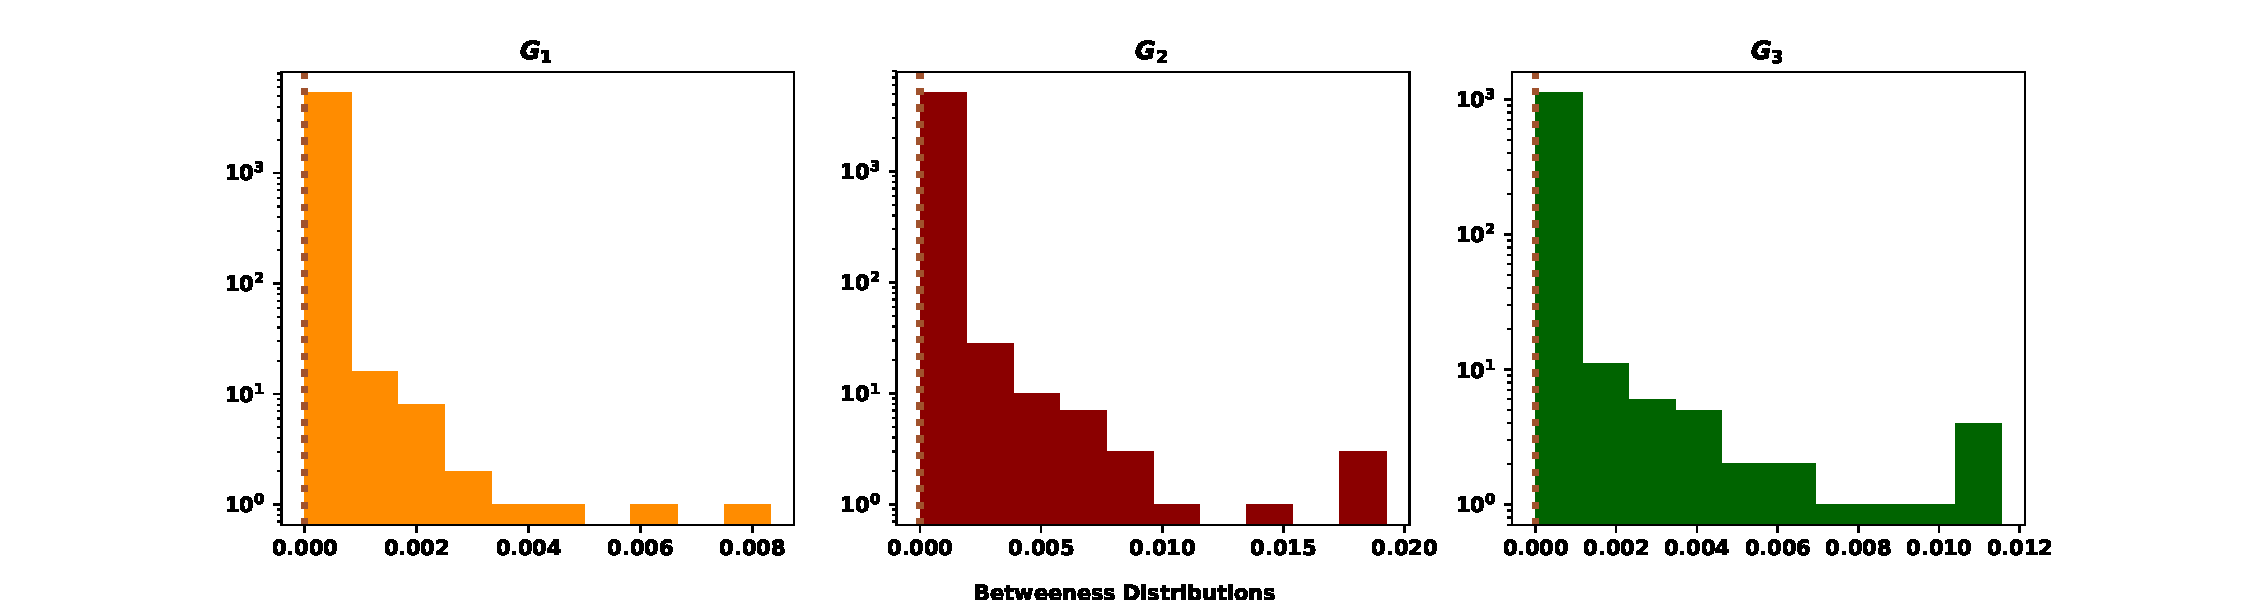
\includegraphics[width=\textwidth]{./assets/images/betweeness_distributions.pdf}
        \caption{Betweenness centrality distributions \(G_1, G_2, G_3\). The descriptive
        statistics for each of the distribution are for \(G_1\): mean\(=0.000019\),
        median\(=0.0\), std\(=0.000207\). For \(G_2\): mean\(=0.000086\), median\(=0.0\),
        std\(=0.000693\) and for \(G_3\): mean\(=0.000151\), median\(=0.0\), std\(=0.000931\).
        None of the three distributions is normally distributed and there is
        significant difference between the means (these have been tested using
        appropriate statistical difference). According to a Mann Whitney both
        \(G_2\) and \(G_3\) medians are significant larger than that of \(G_1\) however there
        is not statistical difference between those two medians.}\label{fig:betweenness_dist}
    \end{subfigure}
    \begin{subfigure}{\textwidth}\centering
        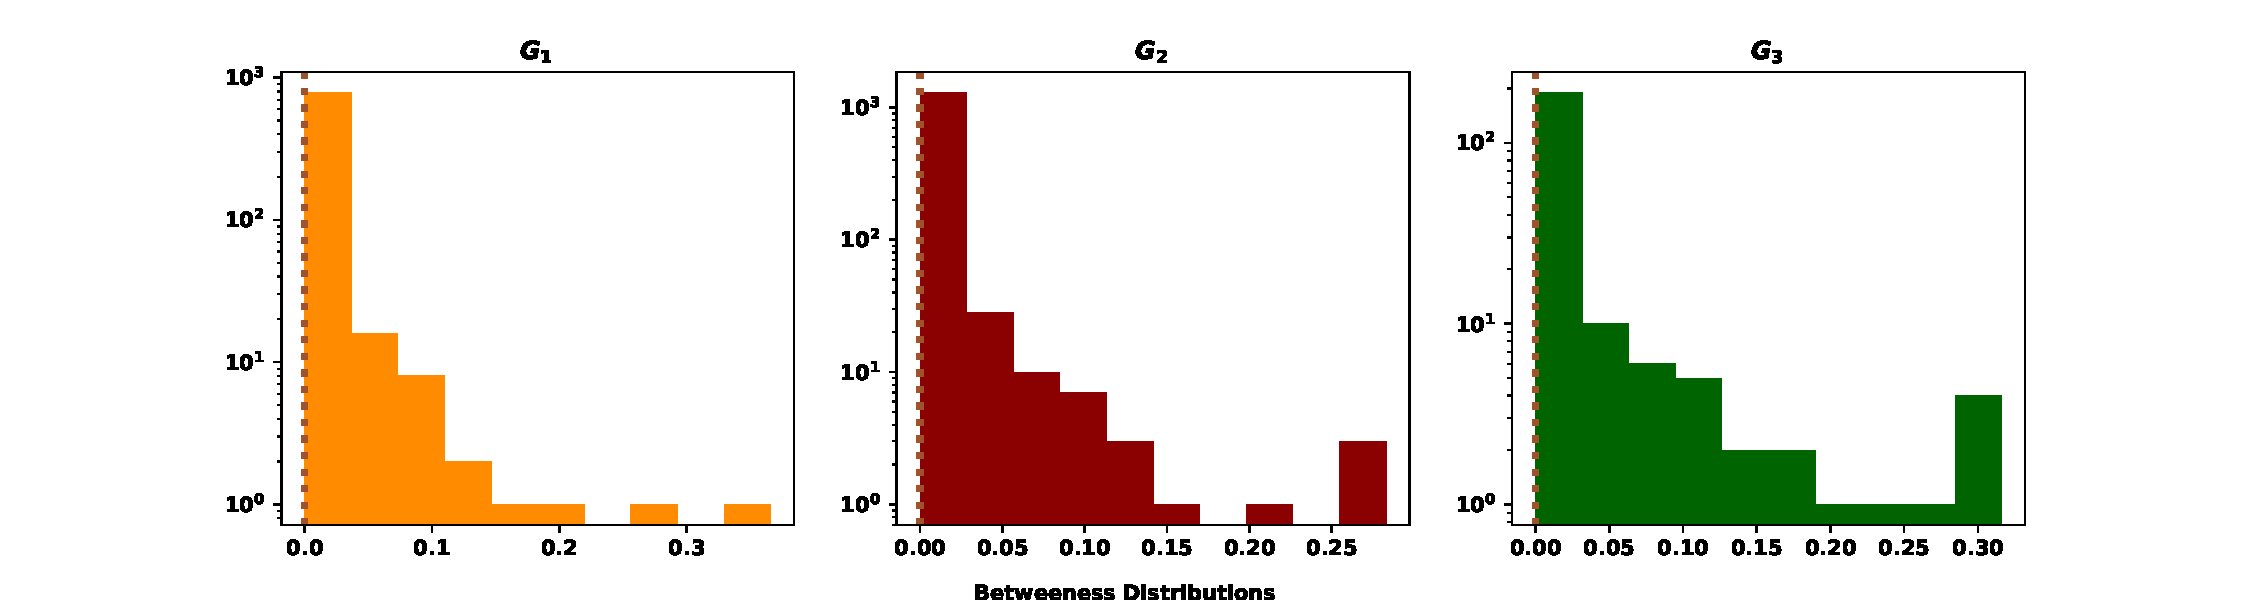
\includegraphics[width=\textwidth]{./assets/images/betweeness_distributions_clusters.pdf}
        \caption{Betweenness centrality distributions for \(G_1, G_2, G_3\) respective
        main clusters.The descriptive
        statistics for each of the distribution are for \(G_1\): mean\(=0.0054\),
        median\(=0.0\), std\(=0.022\). For \(G_2\): mean\(=0.0048\), median\(=0.0\),
        std\(=0.019\) and for \(G_3\): mean\(=0.02\), median\(=0.0\), std\(=0.055\).
        None of the three distributions is normally distributed. There is no
        statistical difference between the medians of \(G_1\) and \(G_3\). There
        is however, statistical difference between the median of \(G_2\).
        These have been tested using a Kruskal Wallis test.}\label{fig:betweenness_dist_cluster}
    \end{subfigure}
    \caption{}
\end{figure}

In relation to influencing your field. An author is most likely to influence their
field if they write for the price of anarchy and authors that publish on auctions
game are more likely to influence compared to authors in the IPD.
Though if an author was to be placed in the main cluster of the respective
field they would chose to be in either \(G_1\) or \(G_3\).
In conclusion, authors regarding both influence metrics that have been defined here
are more likely to gain more if they were to published on either topics of auction
games or the price of anarchy. Though the value of gaining is actual small,
you are more likely to influence your field more in another field compared to that
of the PD.

\begin{figure}[!hbtp]
    \centering
    \begin{subfigure}{\textwidth}\centering
    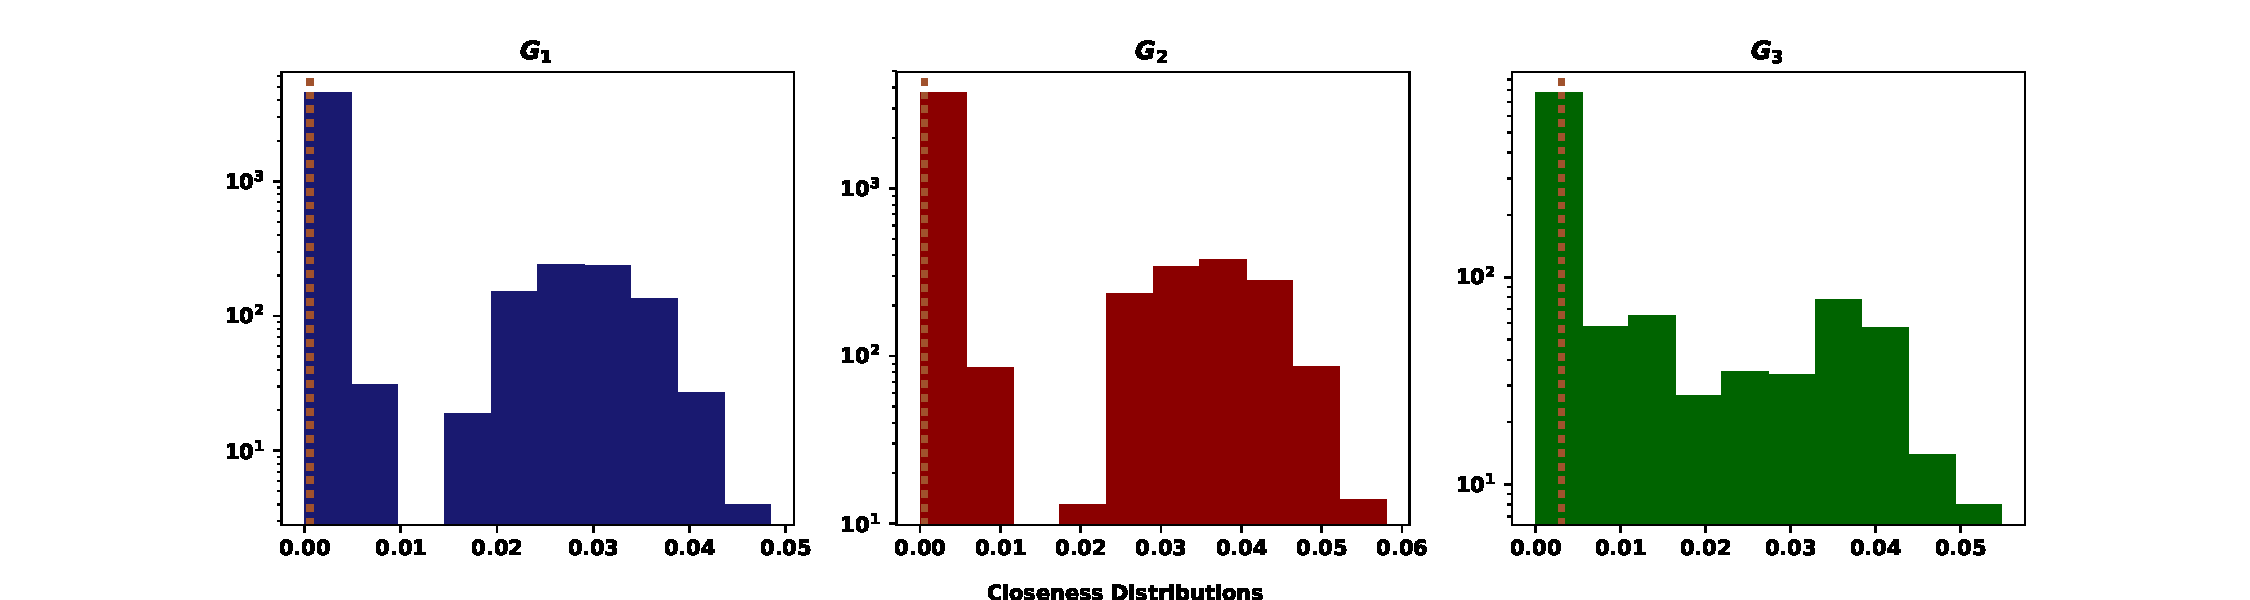
\includegraphics[width=\textwidth]{./assets/images/closeness_distributions.pdf}
    \caption{Closeness centrality distributions \(G_1, G_2, G_3\). The descriptive
        statistics for each of the distribution are for \(G_1\): mean\(=0.0050\),
        median\(=0.00056\), std\(=0.010\). For \(G_2\): mean\(=0.000086\), median\(=0.00058\),
        std\(=0.000693\) and for \(G_3\): mean\(=0.000151\), median\(=0\), std\(=0.000931\).
        None of the three distributions is normally distributed and the median
        of \(G_3\) is statistically larger than that of \(G_2\), which is
        larger than that of \(G_1\).}\label{fig:closeness_dist}
\end{subfigure}
\begin{subfigure}{\textwidth}\centering
    \centering
    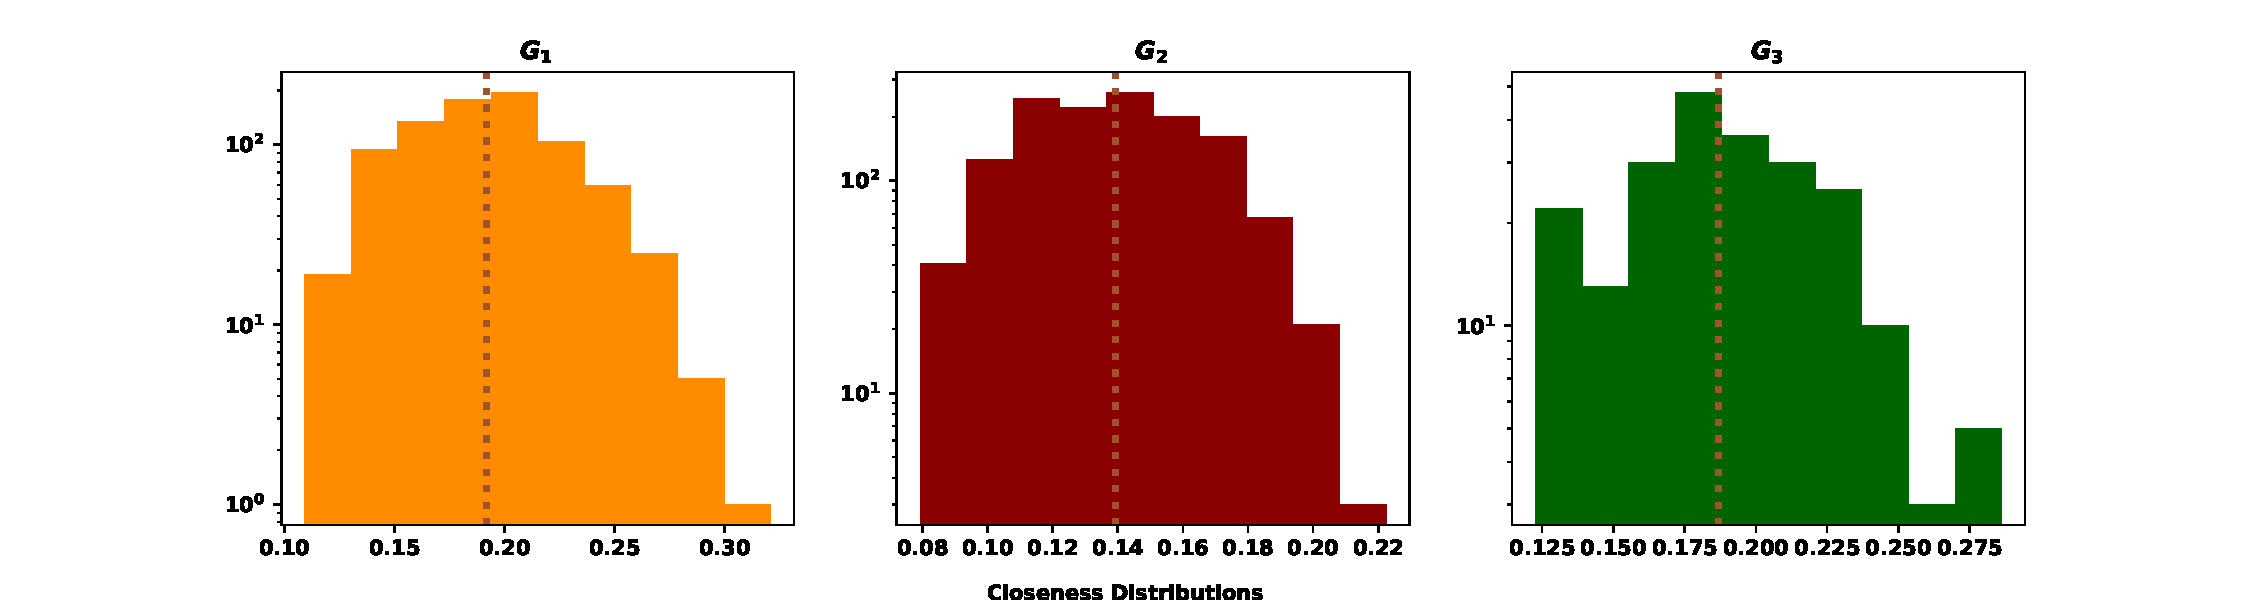
\includegraphics[width=\textwidth]{./assets/images/closeness_distributions_clusters.pdf}
    \caption{Closeness centrality distributions for \(G_1, G_2, G_3\) respective
    main clusters. The descriptive statistics for each of the distribution are
    for \(G_1\): mean\(=0.19\),
    median\(=0.19\), std\(=0.035\). For \(G_2\): mean\(=0.14\), median\(=0.14\),
    std\(=0.026\) and for \(G_3\): mean\(=0.19\), median\(=0.19\), std\(=0.035\).
    None of the three distributions is normally distributed. All medians
    are statistically different. The medians of \(G_1\) and \(G_3\) are greater
    than that of \(G_2\).}\label{fig:closeness_dist_cluster}
    \end{subfigure}
    \caption{}
\end{figure}

\section{Conclusion}

This manuscript presented a coherent literature review on the Iterated
Prisoner's Dilemma. The opening sections focused on research trends and
published works of the field. This was followed by a
presentation of research and educational software. The later sections presented a
meta analysis of publications with the aim of examining the collaborativeness of
the authors and their influence in the research of the game.

The research trends covered in this manuscript included the early experiments
using human subject research, the investigation of cooperative behaviour and the
search of dominant strategies for the game. Human subject research had
limitations and thought it is used by several researchers to date they have
been gradually replaced by the computer tournaments introduced by Axelrod in
1980s. The search of strategies includes strategies that have been manually
designed by an intelligent design and strategies that have been found by
training processes of structures such as finite state automata and neural
networks. Moreover, cooperative behaviour and it's emergence under natural
section was discussed in Section~\ref{subsection:evolutionary_dynamics}.
The results of several milestones have been summarised in this review. These
included the emerge of cooperation in the PD in structured populations, the success
and deficiency of the infamous Tit For Tat, and the training of complex strategies
that evolved a handshake mechanism to combat invasion.

The meta analysis which was covered in the second part of this paper explored
the number of publications, the authors collaborative behaviour and influence in
the research field of the Iterated Prisoner's Dilemma. More than 3000
publications were automatically collected from five different journals. A time
series analysis predicted a continuous growth to the number of publications in
the following years. Moreover, the authors of these papers were used to create a
co authorship network which was studied to compare the field to two other
prominent sub fields of game theory. The results of the analysis showed that the
Iterated Prisoner's Dilemma field is more collaborative than the fields of
auction games and the price of anarchy. However, regarding influence authors are more
likely to have influence more if they were to published on auction games or the
price of anarchy.


\section{Acknowledgements}

A variety of software have been used in this work:

\begin{itemize}
    \item The Axelrod library for IPD simulations~\cite{axelrodproject}.
    \item The Matplotlib library for visualisation~\cite{hunter2007matplotlib}.
    \item The Numpy library for data manipulation~\cite{walt2011numpy}.
    \item The Networkx~\cite{networkx} package for analysing networks.
    \item Gephi~\cite{ICWSM09154} open source package for visualising networks.
    \item The louvain library for calculating the networks modularity.
\end{itemize}

\newpage
\bibliographystyle{plain}
\bibliography{bibliography.bib}
\end{document}